%%% DOCUMENTCLASS %%%%%%%%%%%%%%%%%%%%%%%%%%%%%%%%%%%%%%%%%%%%%
%
\documentclass[10pt, a4paper]{scrartcl}
%
% Optionen f�r {}
%
% scrartcl - Artikel mit europ�ischer Layout-Anpassnug
% scrreprt - Artikel mit europ�ischer Layout-Anpassnug
% scrbook - Buch mit europ�ischer Layout-Anpassnug
% scrlettr - Briefe
%
% Kapitelstruktur: chapter (nur report/book) - section - subsection - subsubsection
%
%
% Optionen f�r []
% 10pt|12pt|14pt - Schriftgr��e
% a4paper - DIN A4
% fleqn - Linksb�ndige statt zentrierte Ausrichtung mathematischer Formeln
% leqno - Gleichungsnummerierungen links statt rechts
% titlepage|notitlepage - Eigene Seite f�r Titel/Zusammenfassung verwenden; Standardeinstellung f�r report/book: titlepage
% onecolumn|twocolumn - Ein- oder zweispaltiges Layout; nicht f�r letter/slides verf�gbar
% oneside|twoside - Ein- oder zweiseitiger Druck; Standard f�r alles au�er book: oneside
%
%
%
%%% DIVERSE PAKETE %%%%%%%%%%%%%%%%%%%%%%%%%%%%%%%%%%%%%%%%%%%%
%
\usepackage[a4paper]{geometry}		% Papierformat
\usepackage[OT2, T1]{fontenc}			% Vektorschriften werden hiermit seltsam rasterm��ig dargestellt ...
\usepackage{lmodern}				% ... jetzt nicht mehr
\usepackage[latin9]{inputenc}			% Codierung der Eingabe; hier: Latin9/ISO-8859-15
\usepackage[english]{babel}			% "ngerman, english": Silbentrennung englisch + neue deutsche Rechtschreibung
\usepackage{amsmath, amssymb, amstext}	% Verbesserte Formeldarstellung, erweiterte mathematischer Zeichenvorrat, \text{}
\usepackage{makeidx} \makeindex		% Index erstellen; Eintrag erstellen mit \index{Bezeichnung[!Unterbezeichnung[!Unterunterbezeichnung]]}; Index schreiben mit \printindex
%

\usepackage{tikz}
\usetikzlibrary{matrix,arrows}

\usepackage{hyperref}
\hypersetup{colorlinks=true, urlcolor=blue}

%
%
% 20110714 EY
\oddsidemargin-0.85cm
\evensidemargin-0.55cm
\topmargin-2.05cm     %I recommend adding these three lines to increase the 
\textwidth18.65cm   %amount of usable space on the page (and save trees)
\textheight25.45cm  
\parindent0.0em
%
%%% SILBENTRENNUNG %%%%%%%%%%%%%%%%%%%%%%%%%%%%%%%%%%%%%%%%%%%%
%
%\hyphenation{Bei-spiel} % Definiert eine selbstdefinierte kontextabh�ngige Silbentrennung im gesamten Dokument; F�r einzelne Flie�textw�rter: Bei\-spiel
%
%%% KOPF- UND FU�ZEILEN %%%%%%%%%%%%%%%%%%%%%%%%%%%%%%%%%%%%%%%
%
\usepackage{scrpage2}
\pagestyle{scrheadings}
\clearscrheadfoot
\usepackage{lastpage}

\automark[subsection]{section}
\ihead{\headmark}
\ohead{\pagemark}
\setheadsepline{1pt}

\pagestyle{plain}


%\theoremstyle{plain}
%\newtheorem{theorem}{Theorem}
%\newtheorem{axiom}{Axiom}
\newtheorem{lemma}{Lemma}
%\newtheorem{proposition}{Proposition}
%\newtheorem{corollary}{Corollary}

%\theoremstyle{definition}
%\newtheorem{definition}{Definition}



%\documentclass[twoside]{amsart}
%\usepackage{amssymb,latexsym}
%\usepackage{MnSymbol}
%\usepackage{times}
%\usepackage{graphics}
%\usepackage{tikz}
%\usepackage{hyperref}
%\hypersetup{colorlinks=true, urlcolor=blue}
%\usepackage{simpsons}
%\usepackage{epsdice}
%\usepackage{staves} 

%\usetikzlibrary{matrix,arrows}
%\usepackage{graphics}

%\oddsidemargin-0.85cm
%\evensidemargin-0.65cm
%\topmargin-2.05cm     %I recommend adding these three lines to increase the 
%\textwidth19.05cm   %amount of usable space on the page (and save trees)
%\textheight25.05cm  
%\parindent0.0em

%This next line (when uncommented) allow you to use encapsulated
%postscript files for figures in your document
%\usepackage{epsfig}

%plain makes sure that we have page numbers





%\chead{}
%\ihead{ssad}
%\cfoot{\pagemark/\pageref{LastPage}}
%\usepackage{fancyhdr}
%%\pagestyle{fancy}
%\fancyhead[L]{}
%\fancyhead[C]{--~\thepage~--}
%\fancyhead[R]{}
%\fancyfoot[L]{}
%\fancyfoot[C]{}
%\fancyfoot[R]{}
%
%%% SONSTIGES %%%%%%%%%%%%%%%%%%%%%%%%%%%%%%%%%%%%%%%%%%%%%%%%%
%

\setcounter{secnumdepth}{-1}
% -1 keine �berschrift wird nummeriert
% 0 Kapitel�berschriften (oder Abschnitts�berschriften im article.sty) werden nummeriert
% 1 die beiden h�chsten Ebenen werden nummeriert
% 5 alle �berschriften werden nummeriert. (Die Werte 2, 3, 4 ergeben die Zwischenwerte)
% \linespread{} % Zeilenabstand als Vielfaches von 1

\usepackage{tensor}
%	Full documentation: http://ftp.uni-erlangen.de/mirrors/CTAN/macros/latex/contrib/tensor/tensor.pdf
%	Usage of tensor package:
%	Indices only: \indices{^a_{bc}}
%	Tensor: \tensor[indices before]{tensor name}{indices after}
%
\usepackage{cancel} % usage: [\cancel \bcancel \xcancel \cancelto{}]{text}
%
\usepackage{color}
\definecolor{grey}{rgb}{0.6,0.6,0.6}






% CUSTOM(IZED) COMMANDS
\renewcommand{\d}{\mathrm d}                                     % differential
\newcommand{\tdq}[2]{\frac{\d #1}{\d #2}}                        % total differential quotient
\newcommand{\pdq}[2]{\frac{\partial #1}{\partial #2}}            % partial differential quotient
\newcommand{\vpdq}[1]{\frac{\vec\partial}{\vec\partial #1}}      % bold partial differential quotient
\newcommand{\vdq}[2]{\frac{\delta #1}{\delta #2}}                % variational differential quotient
\newcommand{\beq}[1]{\begin{align*}#1\end{align*}}               % block equation without numbering
\newcommand{\beqN}[1]{\begin{align}#1\end{align}}                % block equation with numbering. Use \notag to suppress numbering the numering locally.
\newcommand{\ieq}[1]{\(#1\)}                                     % inline equation
\newcommand{\cross}{\times}                                      % cross product
\renewcommand{\vec}[1]{\boldsymbol{\mathrm{#1}}}                 % print vectors bold/non-italic
\newcommand{\vol}{\operatorname{vol}}                            % volume form
\renewcommand{\inf}{\infty}                                      % infinity
\newcommand{\FT}{\mathcal F}                                     % Fourier transformation
\newcommand{\iFT}{\mathcal F^{-1}}                               % inverse Fourier transformation
\newcommand{\infint}{\int_{-\inf}^\inf}                          % integral from -inf to inf
\newcommand{\refTheorem}[1]{\{\ref{#1}\}}
\newcommand{\refEqn}[1]{(\ref{#1})}
\renewcommand{\i}{\mathrm i}                                     % imaginary unit
\renewcommand{\H}{\mathcal{H}}                                   % Hamiltonian
\renewcommand{\L}{\mathcal{L}}                                   % Lie derivative

% Redefinition of basic functions so parentheses are automatically added
\newcommand\nfunc[2]{\operatorname{#1}\left(#2\right)}           % named function
%\renewcommand\exp[1]{\nfunc{exp}{#1}}                            % exp
\renewcommand\sin[1]{\nfunc{sin}{#1}}                            % sin
\renewcommand\cos[1]{\nfunc{cos}{#1}}                            % cos
\renewcommand\tan[1]{\nfunc{tan}{#1}}                            % tan
\renewcommand\cot[1]{\nfunc{cot}{#1}}                            % cot
\renewcommand\Re[1]{\nfunc{Re}{#1}}                              % Re
\renewcommand\Im[1]{\nfunc{Im}{#1}}                              % Im
\newcommand\Res[1]{\nfunc{Res}{#1}}                              % Res
\renewcommand\div[1]{\nfunc{div}{#1}}                            % div
\newcommand\grad[1]{\nfunc{grad}{#1}}                            % grad
\newcommand\curl[1]{\nfunc{curl}{#1}}                            % curl
\newcommand\rot[1]{\nfunc{rot}{#1}}                              % rot = curl
\newcommand\sign[1]{\nfunc{sign}{#1}}                            % rot = curl
\renewcommand\deg[1]{\nfunc{deg}{#1}}                            % degree
\newcommand\supp[1]{\nfunc{supp}{#1}}                            % support
\newcommand\tr[1]{\nfunc{Tr}{#1}}                                % trace
\renewcommand\det[1]{\nfunc{det}{#1}}                            % determinant
\usepackage{dsfont}\newcommand{\unity}{\mathds{1}}               % identity matrix/operator
\newcommand{\identical}{\equiv}                                  % identical

%\renewcommand{\matrix}[1]{\begin{matrix}#1\end{matrix}}          % matrix without parentheses
\newcommand{\matrixp}[1]{\begin{pmatrix}#1\end{pmatrix}}         % matrix with normal braces
\newcommand{\Cases}[1]{\begin{cases}#1\end{cases}}               % piecewise functions etc
\newcommand{\const}{\mathrm{const.}}







% Cyrillic stuff
% thought to be used in mathmode
\newcommand\cyrillic[1]{{\fontencoding{OT2}\fontfamily{wncyr}\selectfont #1}}
\newcommand\mathcyr[1]{\text{\cyrillic{#1}}}
                                    % a     (identical to a)
                                    % A     (identical to A)
\newcommand\be{\mathcyr{b}}         % be    (resembles delta)
\newcommand\Be{\mathcyr{B}}         % Be    (resembles b)
\newcommand\ve{\mathcyr{v}}         % ve    (small B)
                                    % Ve    (identical to B)
\renewcommand\ge{\mathcyr{g}}       % ge    (small Gamma)
                                    % Ge    (identical to Gamma)
\newcommand\de{\mathcyr{d}}         % de    (somewhat edgy-A-looking)
\newcommand\De{\mathcyr{D}}         % De    (larger version of de)
                                    % ye    (identical to e)
                                    % Ye    (identical to E)
\newcommand\zhe{\mathcyr{zh}}       % zhe   (resembles asterisk)
\newcommand\Zhe{\mathcyr{Zh}}       % Zhe   (larger version of zhe)
                                    % dze   (identical to s)
                                    % Dze   (identical to S)
                                    % ze    (almost identical to 3)
                                    % Ze    (larger version of ze)
\newcommand\invn{\mathcyr{i}}       % -     (inverted N)
\newcommand\Invn{\mathcyr{I}}       % -     (larger version of invn)
                                    % k     (identical to kappa)
                                    % K     (identical to Kappa)
\newcommand\el{\mathcyr{l}}         % el    (resembles pi)
\newcommand\El{\mathcyr{L}}         % El    (resembles Pi)
\newcommand\emm{\mathcyr{m}}        % em    (small M)
                                    % Em    (identical to M)
\newcommand\en{\mathcyr{n}}         % en    (small N)
                                    % En    (identical to N)
                                    % o     (identical to o)
                                    % O     (identical to O)
\newcommand\pe{\mathcyr{p}}         % pe    (small Pi)
                                    % Pe    (identical to Pi)
                                    % koppa (identical to c)
                                    % Koppa (identical to C)
                                    % er    (identical to p)
                                    % Er    (identical to P)
\newcommand\te{\mathcyr{t}}         % te    (small T)
                                    % Te    (identical to T)
                                    % tshe  (identical to hbar)
\newcommand\Tshe{\mathcyr{C1}}      % Tshe  (T+h)
                                    % ef    (almost identical to varphi)
                                    % Ef    (identical ti Phi)
                                    % kha   (identical to x)
                                    % Kha   (identical to X)
\newcommand\tse{\mathcyr{ts}}       % tse   (small upside-down Pi with some kind of a hook)
\newcommand\Tse{\mathcyr{Ts}}       % Tse   (larger version of tse)
\newcommand\che{\mathcyr{ch}}       % che   (turn h by 180�)
\newcommand\Che{\mathcyr{Ch}}       % Che   (larger version of che)
\newcommand\sha{\mathcyr{sh}}       % sha   (small upside-down triple pi)
\newcommand\Sha{\mathcyr{Sh}}       % Sha   (larger version of sha)
\newcommand\shta{\mathcyr{shch}}    % shta  (sha with hook)
\newcommand\Shta{\mathcyr{Shch}}    % Shtaa (Sha with hook)
\newcommand\yer{\mathcyr{p2}}       % yer   (hard sign, small b with a hook)
\newcommand\Yer{\mathcyr{P2}}       % Yer   (larger version of yer)
                                    % yeri  (bI. that's two characters. gtfo.)
                                    % yat   (more b with more hooks, no, i'm out)
\newcommand\yu{\mathcyr{yu}}        % yu    (|-O)
\newcommand\Yu{\mathcyr{Yu}}        % Yu    (larger version of yu)
\newcommand\ya{\mathcyr{ya}}        % ya    (mirrored R)
\newcommand\Ya{\mathcyr{Ya}}        % Ya    (larger version of ya)
% test all letters: \be\Be\ve\ge\de\De\zhe\Zhe\invn\Invn\el\El\em\en\pe\te\Tshe\tse\Tse\che\Che\sha\Sha\shta\Shta\yer\Yer\yu\Yu\ya\Ya
% end cyrillic stuff

% enabled by package amsthm
\newtheorem{theorem}{Theorem}
\newtheorem{corollary}[theorem]{Corollary}
\newtheorem{definition}[theorem]{Definition}



\begin{document}


\title{The Geometry of Physics --\\Problem Solutions}
\author{David Luposchainsky, Ernest Yeung}
\date{\number\day.\,\number\month.\,\number\year}
\maketitle

\abstract{These are my solutions to problems given in Theodore Frankel's book ``The Geometry of Physics'' (second edition). As I could not find any other sources, I do not know whether they are correct or not, so read with care (especially the index battles). If you have a solution that is not in here already, a better way of showing something, or just some useful comment, I'd like to hear about it\footnote{e-mail: stupid underscore name at gmx dot net}.} \\

20110714 - further solutions begun by Ernest Yeung.


\section*{Conventions}
If not mentioned differently, use the following conventions:
\begin{itemize}
	\item Use Einstein summation. Sometimes I'll typeset a \(\sum\) for clarification though.
	\item The ``\(\rightharpoondown\)'' used in the book will be used implicitly, i.e. multiindices are always assumed to be in ascending order.
	%\item Abbreviations concerning the metric tensor: \\ \ieq{g:=|\det{\{g_{ij}\}}|}, \ieq{s:=\sign{\det{\{g_{ij}\}}}}
\end{itemize}

\newpage

\setcounter{tocdepth}{4}
\tableofcontents

\newpage

\section*{I Manifolds, Tensors and Exterior Forms}
                   
\section{Manifolds and Vector Fields}
 % 01ManifoldsVector.tex

\subsection{Submanifolds of Euclidean Space}

\paragraph{1.1(3)}

Consider for $F(A) = \det{A}$, $F:\mathbb{R^{n^2}} \to \mathbb{R}$, that 
\[
\begin{gathered}
  \det{A + tB } = \det{ A ( 1 + tA^{-1} B)  } = \det{A} \det{  1 + tA^{-1}B}
\end{gathered}
\]

How to deal with $\det{1 + tA^{-1}B}$?  Recall that 
\[
\det{  1 + tA^{-1}B} = \det{A} ( 1 + t\tr{A^{-1} B})
\]
because for $ \det{(1 + tX)}$, 

\[
\begin{gathered}
  \det{(1+ tX)} = \det{  \matrixp{1& & \\ &\ddots & \\ && 1 }  +  \matrixp{ t x_{11} & \dots & t x_{1n} \\ \vdots & \ddots & \vdots \\ tx_{n1} & \dots & t x_{nn} }   } = 
  \det{  \matrixp{ 1 + tx_{11}& \dots & tx_{1n } \\ 
      \vdots & \ddots & \vdots \\ 
      tx_{n1} & \dots & 1 + tx_{nn}} } = \\
  = 1 + t\tr{X} + \mathcal{O}(t^2)
\end{gathered}
\]
since recall $\det{A} = \sum_{\sigma \in S_n} \text{sgn}{(\sigma)} A_{1 \sigma_1} A_{2\sigma_2} \dots A_{n\sigma_n}$, where sum is over all permutations of $\lbrace 1, \dots, n \rbrace$, and so only the $A_{11}\dots A_{nn}$ term would have terms of $\mathcal{O}(t)$.  

So
\[
(DF) \cdot B = \frac{d}{dt}  F(x(t)) B = \det{x} \tr{x^{-1} B}
\]
For $x_0 \in Sl(n)$, $\det{x_0} = 1$.  Let $B = \frac{r}{n} x$.  Then 
\[
(DF)\cdot B = \tr{x^{-1} \frac{r}{n} x  } = r 
\]
$DF = F_*$ is surjective $\forall \, x \in Sl(n)$


\subsection{Manifolds}



\subsection{Tangent Vectors and Mappings}

\subsubsection{ Tangent or ``Contravariant Vectors}

\subsubsection{ Vectors as Differential Operators}



\subsubsection{ The Tangent Space to $M^n$ at a Point }


\subsubsection{ Mappings and Submanifolds of Manifolds}


\begin{definition} $M^m \subset N^n$ (embedded) submanifold of $N^n$.  If $M$ locally s.t. $F: N^n \to \mathbb{R}^{n-m}$ 
\[
\begin{aligned}
  & F^1(x^1 \dots x^n) = 0 \\ 
  & \vdots \\ 
  & F^{n-m}(x^1 \dots x^n) = 0 
\end{aligned}
\]
$n-m$ diff. $F^i$ s.t. $\left| \frac{ \partial F^i}{ \partial x^j} \right| $ has rank $n-m$
\end{definition}

By implicit function thm., submanifold as graph.  
\[
\begin{gathered}
  (x^1 \dots x^m, y^{m+1} \dots y^n ) \\ 
  \begin{aligned}
    & y^{m+1} = f^{m=1}(x^1 \dots x^m)  \\ 
    & \vdots \\ 
    & y^n = f^n(x^1 \dots x^m)
\end{aligned}
\end{gathered}
\]

on $F(x) = 0$ 

\begin{theorem}[1.12] Let $F: M^m \to N^n$, $q \in N^n$ s.t. $F^{-1}(q) \subset M^m $, $F^{-1}(q) \neq \emptyset$ \\
If $F_*$ onto, i.e. $F_*$ rank $n$, $\forall \, F^{-1}(q)$, \\
$F^{-1}(q)$ ($n-m$)-dim. submanifold of $M^m$
\end{theorem}




\subsubsection{ Change of Coordinates}




                                                                  
\section{Tensors and Exterior Forms}
		\subsubsection{2.1 Covectors and Riemannian Metrics}

\paragraph{2.1(1)}

\textbf{Want}: $ \sum a_i^V v_V^i = \sum a_j^U v^j_U$
\[
a^U_i dx_U^i(v) = a_i^U dx_U^i\left( v_U^j \frac{ \partial }{ \partial x^j_U} \right) = a_i^U v_U^i = a_i^V dx_V^i(v) = a_i^V dx_V^i \left( v^j_V \frac{ \partial }{ \partial x^j_V } \right) = a_i^V v_V^i
\]
or 
\[
a_j^U v_U^j = a_i^V \frac{ \partial x_V^i }{ \partial x_U^j } v^j_U = a_i^V \frac{ \partial x_V^i }{ \partial x_U^j } \frac{ \partial x^j_U }{ \partial x_V^k}(p_0) v_V^k = a_i^V v^i_V
\]
were (1.6) was used.  

\[
v^i w^i = v^i_U w^i_U = \frac{ \partial x^i_U}{\partial x_V^j} v^j_V \frac{ \partial x_U^i }{ \partial x^k_V} w_V^k = \frac{ \partial x^i_U}{ \partial x^j_V } \frac{ \partial x_U^i }{ \partial x^k_V} v_V^j w_V^k 
\]
transforms as a $(0,2)$ tensor.  

\paragraph{2.1(2)}
\begin{enumerate}
\item[(i)] 
Recall \[
g_{ij}^V = \frac{ \partial x^r_U}{ \partial x_V } \frac{ \partial x_U^s}{ \partial x_V^j } g_{rs}^U
\]
\[
\begin{aligned}
        u^1 & = r \\ 
        u^2 & = \theta \\ 
        u^3 & = \phi
\end{aligned} \quad \begin{aligned} x & = r \cos{\phi} \sin{\theta} \\ 
              y & = r \sin{\phi} \sin{\theta} \\
              z & = r\cos{\theta} \end{aligned} \quad 
\begin{aligned}
\frac{ \partial x}{ \partial r } & = c{\phi} s{\theta} \\ 
       \frac{ \partial y}{ \partial r } & = s{\phi} s{\theta} \\ 
       \frac{ \partial z }{ \partial r } & = c{\theta} 
\end{aligned}
\quad 
\begin{aligned}
\frac{ \partial x}{ \partial \theta} & = r c{\phi} c{\theta} \\ 
      \frac{ \partial y }{ \partial \theta} & = r s{\phi} c{\theta}  \\
      \frac{ \partial z}{ \partial \theta} & = -r s{\theta} 
\end{aligned} \quad 
\begin{aligned}
\frac{ \partial x}{ \partial \phi} &=  -r s{\phi} s{\theta} \\ 
       \frac{ \partial y}{ \partial \phi} & = rc{\phi} s{\theta} \\
       \frac{ \partial z}{ \partial \phi} & = 0 \end{aligned}
\]
\[
\boxed{ 
\begin{aligned}
g_{rr} & = 1 \\
g_{\theta \theta} & = r^2 \\
g_{\phi \phi} & = r^2 (\sin{\theta})^2
\end{aligned} }
\]
\item[(ii)] $\grad{f} = \nabla f$ is contravariant vector, associated to covector $df$, \, $df(w) = \langle \nabla f, w \rangle$.  $(\nabla f)^i = g^{ij} \frac{ \partial f}{ \partial x^j}$  \\

$g^{ij}$ is \textbf{not} $g_{ij}$.  What is $g^{ij}$?

Also $(r, \theta , \phi)$ is a non-coordinate bases.  
\[
ds^2 = (dr)^2 + r^2 (d\theta)^2 + r^2 (\sin{\theta})^2 (d\phi)^2 
\]

The distance elements are $dr$, $rd\theta$, $r\sin{\theta} d\phi$ in this non-coordinate basis $\widehat{r}, \widehat{\theta}, \widehat{\phi}$.  \\
We're using $ds^2 = |d\vec{x}|^2  \equiv g(d\vec{x}, d\vec{x}) = d\vec{x} \cdot d\vec{x}$ instead of $ds^2 = g_{\mu \nu} dx^{\mu} dx^{\nu}$ \\

In the non-coordinate basis $\lbrace \widehat{r}, \widehat{\theta}, \widehat{\phi} \rbrace$.  Coordinate basis $\lbrace \vec{e}_r, \vec{e}_{\theta}, \vec{e}_{\phi} \rbrace$ \\
Consider
\[
g_{\mu' \nu'}  \equiv g(\vec{e}_{\mu'}, \vec{e}_{\nu'} ) = g_{\alpha \beta} \widetilde{e}^{\alpha}(\vec{e}_{\mu'}) \widetilde{e}^{\beta}(\vec{e}_{\nu'} ) = g_{\alpha \beta} \Lambda^{\alpha}_{\, \mu' } \Lambda^{\beta}_{\, \nu' }
\]
\[
g_{\mu \nu} = \vec{e}_{\mu} \cdot \vec{e}_{\nu}
\]
\[
\begin{aligned}
        g_{rr} & = 1 \\ 
        g_{\theta \theta} & = r^2 \\ 
        g_{\phi \phi} & = r^2 (\sin{\theta})^2
\end{aligned}
\]
So $\vec{e}_{\theta} = \frac{ \partial }{ \partial \theta}$, $\vec{e}_{\phi} = \frac{ \partial }{ \partial \phi }$ are \textbf{not unit vectors}!   \\

In the coordinate basis $d\vec{x} = \vec{e}_r dr + \vec{e}_{\theta} d\theta + \vec{e}_{\phi} d\phi = \vec{e}_i dx^i $ \\
In the noncoordinate basis, $d\vec{x} = \widehat{r} dr + \widehat{\theta} r d\theta + \widehat{\phi} r \sin{\theta} d\phi$

\[
\begin{aligned}
        \Lambda^r_{ \, \widehat{r} } & = 1 \\ 
        \Lambda^{\theta}_{\widehat{\theta}} &= \frac{1}{r} \\ 
        \Lambda^{\phi}_{\widehat{\phi}} & = \frac{1}{ r \sin{ \theta}}
\end{aligned}
\]

So then, for instance 
\[
g_{\phi \phi} = r^2 (\sin{\theta})^2 = g(\partial_{\phi}, \partial_{\phi} ) = g_{ij} \widetilde{e}^i (\partial_{\phi}) \widetilde{e}^j(\partial_{\phi}) = g_{ij} \Lambda^i_{\, \phi} \Lambda^j_{\, \phi } = g_{\widehat{\phi} \widehat{\phi}} r^2 (\sin{\theta})^2
\]
\[
\begin{aligned}
        & g_{ \widehat{r} \widehat{r}} = g_{\widehat{\theta} \widehat{\theta}} = g_{\widehat{\phi} \widehat{\phi}} = 1 \\ 
        & g_{\widehat{r} \widehat{\theta}} = g_{\widehat{r} \widehat{\phi} } = g_{\widehat{\theta} \widehat{\phi} } =  0
\end{aligned}
\]

in non-coordinate basis, we must give up the following two:
\[
\begin{aligned}
        & d\vec{x} \equiv dx^{\mu} \vec{e}_{\mu} \text{ defines $\vec{e}_{\mu}$ coordinate basis } \\ 
        & ds^2 = g_{\mu \nu} dx^{\mu} dx^{\nu}
\end{aligned}
\]
Inverse metric components 
\[
\begin{aligned}
        & g^{rr} = 1 \\ 
        & g^{\theta \theta} = \frac{1}{r^2} \\ 
        & g^{\phi \phi} = \frac{1}{ r^2 (\sin{\theta})^2 }
\end{aligned}
\]

The isomorphism of $V$ and $V^*$ (e.g. $T_pM$ and $T_pM^*$) allows us to introduce notation that replaces one-forms with vectors and $(m,n)$ tensors with $(m+n, 0)$ tensors.   \\
Replace basis one-forms $\widetilde{e}^{\mu} \equiv \alpha^{\mu}$ with set of vectors defined
\[
\vec{e}^{\mu}( \cdot ) \equiv g^{-1}(\widetilde{e}^{\mu}, \cdot ) = g^{\mu \nu} \vec{e}_{\mu}(\cdot )
\]
where $\widetilde{e}^{\mu}$ basis one form, $\vec{e}^{\mu}$ dual basis vector.  

Then
\[
\begin{aligned}
        & \vec{e}^r = \vec{e}_r = \frac{ \partial }{ \partial r } = \widehat{r} \\ 
        & \vec{e}^{\theta} = \frac{1}{r^2} \vec{e}_{\theta} = \frac{1}{r} \widehat{\theta} \\ 
        & \vec{e}^{\phi} = \frac{1}{ (r\sin{\theta})^2 } \vec{e}_{\phi} = \frac{1}{ r\sin{\theta} } \widehat{\phi} 
\end{aligned}
\]
Now 
\[
\begin{aligned}
        & \widetilde{\nabla} \equiv \widetilde{e}^{\mu} \partial_{\mu} \, & \text{ in coordinate basis } \\ 
        & \widetilde{\nabla} x^{\mu} = \widetilde{e}^{\mu} \, & \text{ in a coordinate basis } \\
        & \vec{\nabla} = \vec{e}^{\mu} \partial_{\mu} = g^{\mu \nu} \vec{e}_{\mu} \partial_{\nu}
\end{aligned}
\]
So finally
\[
\boxed{ 
\begin{aligned}
        & \vec{\nabla} = \widehat{r} \partial_r + \frac{1}{r} \widehat{\theta} \partial_{\theta} + \frac{1}{ r \sin{\theta}} \widehat{\phi} \partial_{\phi} \\ 
        & \vec{\nabla} f = \widehat{r} \partial_r f + \frac{1}{r} \widehat{\theta} \partial_{\theta} f + \frac{1}{r \sin{\theta}} \widehat{\phi} \partial_{\phi} f 
\end{aligned}
}
\]

Also, in this formulation,
\[
\boxed{
\begin{aligned}
        \vec{\nabla} & = \vec{e}_r \partial_r + \frac{1}{r^2} \vec{e}_{\theta} \partial_{\theta} + \frac{1}{ (r \sin{\theta})^2} \vec{e}_{\phi} \partial_{\phi} \\ 
        \vec{\nabla} f & = \vec{e}_r \partial_r f + \frac{1}{r^2} \partial_{\theta} f \vec{e}_{\theta} + \frac{1}{ (r \sin{\theta})^2 } \partial_{\phi} f \vec{e}_{\phi} = (\partial_r f) \frac{ \partial }{ \partial r } + \frac{1}{r^2} \partial_{\theta} f \frac{ \partial }{ \partial \theta} + \frac{ \partial_{\phi} f}{ (r \sin{\theta})^2} \frac{ \partial }{ \partial \phi} = \\
        & = (\nabla f)^i \partial_i = g^{ij} \frac{ \partial f}{ \partial x^j} \partial_i  
\end{aligned} }
\]
(cf. MIT Physics 8.962 Spring 1999, Edmund Bertschinger.  \textbf{Introduction to Tensor Calculus for General Relativity} \texttt{gr1.pdf})
\item[(iii)] See above.  And as before, 
\[
\begin{aligned}
         \frac{ \partial }{ \partial r } & = \widehat{r} \\ 
         \frac{1}{r} \frac{ \partial }{ \partial \theta}         & = \widehat{\theta} \\ 
       \frac{1}{ r \sin{\theta} }\frac{\partial }{ \partial \phi }  & = \widehat{\phi}
\end{aligned}
\]
\end{enumerate}




\subsubsection{ 2.3. The Cotangent Bundle and Phase Space  }


\paragraph{ 2.3a. The Cotangent Bundle }

\paragraph{ 2.3b. The Pull-Back of a Covector }


\paragraph{ 2.3c. The Phase Space in Mechanics }

Let $q^1 \dots q^m$ local generalized coordinates, $M^m$ configuration space of a dynamical system.  

\[
L: TM^m \to \mathbb{R}
\]
Consider $\begin{aligned} & \quad \\ 
         & (U,q)  \\ & (V,r )  \end{aligned}$, \, $UV \neq \emptyset$, $q\in UV$

$r=r(q)$

\[
\dot{r}^j = \frac{ \partial r^j}{ \partial q^i } \dot{q}^i \quad \quad \quad (2.27) \quad \, \frac{ \partial \dot{r}^j }{ \partial \dot{q}^i } = \frac{ \partial r^j }{ \partial q^i}
\]

\[
\begin{gathered}
\pi_i \equiv \frac{ \partial L}{ \partial \dot{r}^i } = \frac{ \partial L}{ \partial q^j} \frac{ \partial q^j}{ \partial \dot{r}^i } + \frac{ \partial L }{ \partial \dot{q}^j } \frac{ \partial \dot{q}^j }{ \partial \dot{r}^i } = \frac{ \partial L}{ \partial \dot{q}^j } \frac{ \partial \dot{q}^j }{ \partial \dot{r}^i } = \frac{ \partial L}{ \partial \dot{q}^j } \frac{ \partial q^j }{ \partial r^i } \\ 
      \Longrightarrow \pi_i = p_j \frac{ \partial q^j }{ \partial r^i } \quad \quad \quad (2.29)
\end{gathered}
\]

$p$'s are covector.  

\[
\Longrightarrow p : TM^m \to T^*M^m
\]
cotangent bundle.  $T^* M^m $ of covectors to configuration space is phase space.  
\[
\begin{gathered}
        T(q, \dot{q}) = \frac{1}{2} \sum_{jk} g_{jk}(q) \dot{q}^j \dot{q}^k \quad \quad \quad (2.31) \\ 
        p_i = \frac{ \partial L}{ \partial \dot{q}^i } = \frac{ \partial T}{ \partial \dot{q}^i } = \sum_j g_{ij}(q) \dot{q}^j \quad \quad \quad (2.32) 
\end{gathered}
\]

think of $2T$ as Riemannian metric on $M^m$.  
\[
\langle \dot{q}, \dot{q} \rangle = \sum_{ij } g_{ij}(q) \dot{q}^i \dot{q}^j
\]


\paragraph{ 2.3d. The Poincar\'{e} 1-Form}



\subsubsection{2.4 Tensors}

\paragraph{ 2.4a.  Covariant Tensors }

\begin{definition}
        covariant tensor of rank $r$ \\
\[
Q: E \times \dots \times E \to \mathbb{R}
\]
$Q(v_1 \dots v_r)$
\end{definition}

vector space of covariant $r$th rank tensors $E^* \otimes \dots \otimes E^* = \otimes^r E^*$

2nd. rank covariant tensor $\begin{aligned} & \quad \\    
     & \alpha \otimes \beta : E \times E \to \mathbb{R} \\ 
     & \alpha \otimes \beta(v,w) \equiv \alpha(v) \beta(w) \end{aligned}$

\paragraph{2.4(1)}

For any $v, w$ tangent vectors, 
\[
\begin{aligned}
        & v = v^i \frac{ \partial}{ \partial x^i } \\      
        & w = w^i \frac{ \partial}{ \partial x^i } 
\end{aligned}
\]

\[
\begin{gathered}
        ( \alpha \otimes \beta)(v,w) = \alpha(v) \beta(w) = a_i dx^i ( v^j \frac{ \partial }{ \partial x^j} ) b_k dx^k ( w^l \frac{ \partial }{ \partial x^l}  ) = a_i b_k v^j w^l \delta^i_{\, j } \delta^k_{\, l } = a_j v^j b_k w^k = \\
        = a_j b_k dx^j(v) dx^k(w) = a_j b_k dx^j \otimes dx^k(v,w)
\end{gathered}
\]

For $\alpha,\beta$ in components,
\[
\begin{aligned}
        & \alpha = a_i dx^i \\ 
        & \beta = b_j dx^j
\end{aligned}
\]

\[
a_ib_j dx^i \otimes dx^j(v,w) = a_i b_j v^i w^j = a_j v^j b_k w^k \Longrightarrow \alpha \otimes \beta = a_i b_j dx^i \otimes dx^j
 \]

\paragraph{2.4(2)(i)\quad Contraction invariant under base transformation}
\beq{
	\tensor{A}{^\prime^i_i}
	= A(\d x'^i,\vec \partial'_i)
	= A\left(\pdq{x'^i}{x^j}\d x^j,\pdq{x^k}{x'^i} \vec \partial_k\right)
	= \underbrace{\pdq{x'^i}{x^j} \pdq{x^k}{x'^i}}_{\pdq{x^k}{x^j} = \delta^k_j} \underbrace{A\left(\mathrm dx^j,\vec \partial_k\right)}_{= \tensor{A}{^j_k}}
	= \tensor{A}{^j_j}
}
This is the transformation law of a scalar.



\paragraph{2.4(2)(ii)\quad Non-invariant ``contraction''}
\beq{%
	\sum_i A'_{ii}
	&= \sum_i A(\vec \partial'_i, \vec \partial'_i)
	= \sum_i A\left(\pdq{x^j}{x'^i} \vec \partial_j, \pdq{x^k}{x'^i} \vec \partial_k\right)
	= \sum_i \pdq{x^j}{x'^i} \pdq{x^k}{x'^i} \underbrace{A(\vec \partial_j, \vec \partial_k)}_{= A_{jk}} \\
	&= \sum_i \pdq{x^j}{x'^i} \pdq{x^k}{x'^i} A_{jk}
	\neq A_{ii}
}
Since the differential quotients do not cancel out, the value of \(\sum_i A_{ii}\) is dependant on coordinates; a coordinate-dependant number is neither a scalar nor any other sort of tensor.

\paragraph{2.4(3)(i)\quad  Transformation behavior of a contraction}
\beq{
	g'_{ji}v'^i
	= \pdq{x^k}{x'^j} \pdq{x^\ell}{x'^i} g_{k\ell} \pdq{x'^i}{x^m} v^m
	= \pdq{x^k}{x'^j} \underbrace{\pdq{x^\ell}{x'^i} \pdq{x'^i}{x^m}}_{=\delta^\ell_m} g_{k\ell} v^m
	= \pdq{x^k}{x'^j} g_{k\ell} v^\ell
}
Thus, \(g_{ji}v^i\) transforms like a vector.



\paragraph{2.4(3)(ii)\quad  Tensor?}
\beq{
	\partial'_j v'^i
	&= \pdq{}{x'^j} \left(\pdq{x'^i}{x^k} v^k\right)
	= \pdq{^2 x'^i}{x^\ell \partial x^k} \pdq{x^\ell}{x'^j} v^k + \pdq{x'^i}{x^k} \pdq{v^k}{x'^j}
	= \pdq{^2 x'^i}{x^\ell \partial x^k} \pdq{x^\ell}{x'^j} v^k + \pdq{x'^i}{x^k} \underbrace{\pdq{v^k}{x^\ell}}_{= \partial_\ell v^k} \pdq{x^\ell}{x'^j}
	\\
	&= \underbrace{\pdq{^2 x'^i}{x^\ell \partial x^k} \pdq{x^\ell}{x'^j} v^k}_{\neq 0} + \pdq{x^\ell}{x'^j} \pdq{x'^i}{x^k} \partial_\ell v^k
}
Although the second term is the correct tensor transformation law, the first term prevents \(\partial_j v^i\) from forming a tensor.



\paragraph{2.4(3)(iii)\quad  Tensor? -- second attempt}
\ \\
Using the result of (ii), one gets
\beq{
	\partial'_j v'^i - \partial'_i v'^j
	&= \pdq{^2 x'^i}{x^\ell \partial x^k} \pdq{x^\ell}{x'^j} v^k + \pdq{x^\ell}{x'^j} \pdq{x'^i}{x^k} \partial_\ell v^k - \pdq{^2 x'^j}{x^\ell \partial x^k} \pdq{x^\ell}{x'^i} v^k - \pdq{x^\ell}{x'^i} \pdq{x'^j}{x^k} \partial_\ell v^k
	\\
	&= \left(\pdq{^2 x'^i}{x^\ell \partial x^k} \pdq{x^\ell}{x'^j} v^k - \pdq{^2 x'^j}{x^\ell \partial x^k} \pdq{x^\ell}{x'^i} v^k\right) + \left(\pdq{x^\ell}{x'^j} \pdq{x'^i}{x^k} \partial_\ell v^k - \pdq{x^\ell}{x'^i} \pdq{x'^j}{x^k} \partial_\ell v^k\right)
	\\
	&\neq 0 + \pdq{x^\ell}{x'^j} \pdq{x'^i}{x^k} \left(\partial_\ell v^k - \partial_k v^\ell\right)
}

\paragraph{2.4(4)}

\begin{enumerate}
\item[(i)] \[
L = L(q,\dot{q}) = \frac{1}{2} g_{ij}(q) \dot{q}^i \dot{q}^j - V 
\]
\[
\frac{d}{dt} \left( \frac{ \partial L}{ \partial \dot{q}^k} \right) = \frac{ \partial L}{ \partial q^k }
\]

\[
V=V(q) = V(0)  + \frac{ \partial V}{ \partial q^i} q^i + \frac{1}{2} \frac{ \partial^2 V}{ \partial q^i \partial q^j } q^i q^j
\]

Assume $g$ symmetric in indices.  

$\frac{ \partial V}{ \partial q^k} = 0$ i.e. $q=0$ nondegenerate minimum for $V$.

\[
\frac{d}{dt} \left( \frac{ \partial L }{ \partial \dot{q}^i } \right) = g_{ij}(0) \dot{q}^j = -\frac{ \partial^2 V}{ \partial q^i \partial q^j } q^j = -Q_{ij} q^j 
\]



\item[(ii)]
\item[(iii)]
\end{enumerate}



\subsection{2.5 The Gra�mann or Exterior Algebra}

\subsubsection{2.5a. The Tensor Product of Covariant Tensors}

\subsubsection{2.5b. The Grassmann or Exterior Algebra}


\[
\alpha = \alpha_{\underline{J}} dx^{ \underline{J}} = \frac{1}{p!} \alpha_J dx^J
\]
$\alpha_J$ antisymmetric in $J$ and $\alpha_{\underline{J}}$ antisymmetric in $\underline{J}$

\[
\alpha_{\underline{J}}  = p! \alpha_J
\]

\begin{lemma}[2.46]
\[
\delta^{I\underline{J}}_M \delta^{KL}_{\underline{J}} = \delta^{IKL}_M
\]
\end{lemma}
\textbf{Proof}
%\begin{proof}

\[
\begin{aligned}
        & I = (i_1 \dots i_{p} ) \\
        & J = (j_1 \dots j_{q+r} ) \\ 
        & \underline{J} = (j_1 < \dots < j_{q+r}) \\ 
        & K = (k_1 \dots k_q) \\ 
        & L = (l_1 \dots l_r) \\ 
        & M = (m_1 \dots m_{p+q+r} )
\end{aligned}
\]


        $KL$ fixed.  put $KL$ into (unique) increasing order, by as many transpositions as total number of inversions (cf. Tu, L.W., Introduction to Manifolds, Springer, 2008), Proposition 3.6)

so $\delta_{\underline{J}}^{KL} \neq 0$ for only 1 $\underline{J}$

Suppose $\delta_{\underline{J}}^{KL} =1$,  $KL$ even permutation of $\underline{J}$ (permutation is bijective)

$M$ fixed so suppose $I\underline{J}$ even permutation of $M$

$I\sigma(KL) = f(M)$

$\sigma$ even permutation of $KL$, so put $\sigma(KL)$ into $KL$ by even number of transpositions  \\
This defines even permutation $g$ that's bijective on $I\sigma(KL)$
\[
g(I\sigma(KL)) = IKL =gf(M)
\]
so $IKL$ even permutation of $M$. 

If $I\overline{J}$ odd permutation of $M$, $gf$ odd permutation, $\delta_M^{IKL} = -1$


%\end{proof}

\hrulefill

\subsubsection{2.5c. The Geometric Meaning of Forms in $\mathbb{R}^n$}

\paragraph{2.5(1)\quad Basis expansion of a form}
\beq{
	\left(a_J \mathrm dx^J\right)\left(\vec \partial_K\right)
	= a_J \mathrm dx^J \left(\vec \partial_K\right)
	= a_J \delta^J_K
	= a_K
	= \alpha \left(\vec \partial_K\right)
}
Since this is true for all \(\vec \partial_K\), \(\alpha = a_J \mathrm dx^J\).



\paragraph{2.5(2)\quad Components of $\alpha^1\wedge\beta^2$}
\beq{
	(\alpha^1\wedge\beta^2)_{i<j<k} = \sum_{l,m<n}\delta_{ijk}^{lmn}\alpha_l\beta_{mn}
}
All summands where \(ijk\) is not a permutation of \(lmn\) vanish, so there are 6 possible permutations left:

\begin{table}[h]
	\centering
	\begin{tabular}{ccc|ccc|ccc|ccc|ccc|ccc}
		&(A)& & &(B)& & &(C)& & &(D)& & &(E)& & &(F)& \\
		\hline
		i&=&l & i&=&m & i&=&n & i&=&l & i&=&n & i&=&m \\
		j&=&m & j&=&n & j&=&l & j&=&n & j&=&m & j&=&l \\
		k&=&n & k&=&l & k&=&m & k&=&m & k&=&l & k&=&n
	\end{tabular}
\end{table}
Of these 6, (C), (D) and (E) contradict \(i<j<k\) (given by the problem) with respect to \(m<n\) (from the definition of the wedge product), leaving only 3 summands. Thus,
\beq{
	(\alpha^1\wedge\beta^2)_{i<j<k} &= \sum_{l,m<n}\delta_{ijk}^{lmn}\alpha_l\beta_{mn} = \underbrace{\delta_{ijk}^{ijk}}_{(A)\rightarrow+1}\alpha_i\beta_{jk} + \underbrace{\delta_{ijk}^{kij}}_{(B)\rightarrow+1}\alpha_k\beta_{ij} + \underbrace{\delta_{ijk}^{jik}}_{(F)\rightarrow-1}\alpha_j\underbrace{\beta_{ik}}_{-\beta_{ki}} \\
	&= \alpha_i\beta_{jk}+\alpha_j\beta_{ki}+\alpha_k\beta_{ij} \; .
}

\paragraph{2.5(3)}
In $\mathbb{R}^3$, 

Given
\[
\begin{aligned}
        \alpha^1 = a_1 dx^1 + \dots + a_3 dx^3 \\ 
        \beta^1 = b_1 dx^1 + b_2 dx^2 + b_3 dx^3 \\ 
        \rho^1 = r_1 dx^1 + r_2 dx^2 + r_3 dx^3  \\
        \gamma^2 = c_1 dx^2 \wedge dx^3 + c_2 dx^3 \wedge dx^1 + c_3 dx^1 \wedge dx^2
\end{aligned}
\]
\[
\alpha^1 \wedge \gamma^2 = (a_1 c_1 + a_2 c_2 + a_3 c_3 ) dx^1 \wedge dx^2 \wedge dx^3 = a\cdot c dx^1 \wedge dx^2 \wedge dx^3 = a\cdot c \text{vol}{ (dx) }
\]
\[
\begin{gathered}
        \alpha^1 \wedge \beta^1 = (a_1 b_2 - a_2 b_1 ) dx^1 \wedge dx^2 +  ( a_1 b_3 - a_3 b_1) dx^1 \wedge dx^3 + (a_2 b_3 - a_3 b_2 ) dx^2 \wedge dx^3 \\
 \alpha^1 \wedge \beta^1 \wedge \rho^1 = ( (a_1 b_2 - a_2 b_1) r_3 + (-r_2) (a_1 b_3 - a_3 b_1) + r_1(a_2 b_3 - a_3 b_2) ) dx^1 \wedge dx^2 \wedge dx^3 = r\cdot (a\times b) \text{vol}{ (dx) }
\end{gathered}
\]


\subsubsection{2.6 Exterior Differentiation}



\paragraph{2.6(1)\quad Differential of a 3-Form in $\mathbb R^4$}
\beq{
	\beta^3
	&= \beta_J \mathrm dx^J
	= \sum_{i<j<k} \beta_{ijk} \mathrm dx^i \wedge \mathrm dx^j \wedge \mathrm dx^k
	\\
	&=
		  \beta_{123} \mathrm dx^1 \wedge \mathrm dx^2 \wedge \mathrm dx^3
		+ \beta_{124} \mathrm dx^1 \wedge \mathrm dx^2 \wedge \mathrm dx^4
		\\ &\qquad
		+ \beta_{134} \mathrm dx^1 \wedge \mathrm dx^3 \wedge \mathrm dx^4
		+ \beta_{234} \mathrm dx^2 \wedge \mathrm dx^3 \wedge \mathrm dx^4
	\\
	\Rightarrow \mathrm d\beta^3
	&=
		  \mathrm d\beta_{123} \wedge \mathrm dx^1 \wedge \mathrm dx^2 \wedge \mathrm dx^3
		+ \mathrm d\beta_{124} \wedge \mathrm dx^1 \wedge \mathrm dx^2 \wedge \mathrm dx^4
		\\ &\qquad
		+ \mathrm d\beta_{134} \wedge \mathrm dx^1 \wedge \mathrm dx^3 \wedge \mathrm dx^4
		+ \mathrm d\beta_{234} \wedge \mathrm dx^2 \wedge \mathrm dx^3 \wedge \mathrm dx^4
	\\
	&=
		  \pdq{\beta_{123}}{x^i} \; \mathrm dx^i \wedge \mathrm dx^1 \wedge \mathrm dx^2 \wedge \mathrm dx^3
		+ \pdq{\beta_{124}}{x^i} \; \mathrm dx^i \wedge \mathrm dx^1 \wedge \mathrm dx^2 \wedge \mathrm dx^4
		\\ &\qquad
		+ \pdq{\beta_{134}}{x^i} \; \mathrm dx^i \wedge \mathrm dx^1 \wedge \mathrm dx^3 \wedge \mathrm dx^4
		+ \pdq{\beta_{234}}{x^i} \; \mathrm dx^i \wedge \mathrm dx^2 \wedge \mathrm dx^3 \wedge \mathrm dx^4
	\\
	&=
		  \pdq{\beta_{123}}{x^4} \; \mathrm dx^4 \wedge \mathrm dx^1 \wedge \mathrm dx^2 \wedge \mathrm dx^3
		+ \pdq{\beta_{124}}{x^3} \; \mathrm dx^3 \wedge \mathrm dx^1 \wedge \mathrm dx^2 \wedge \mathrm dx^4
		\\ &\qquad
		+ \pdq{\beta_{134}}{x^2} \; \mathrm dx^2 \wedge \mathrm dx^1 \wedge \mathrm dx^3 \wedge \mathrm dx^4
		+ \pdq{\beta_{234}}{x^1} \; \mathrm dx^1 \wedge \mathrm dx^2 \wedge \mathrm dx^3 \wedge \mathrm dx^4
	\\
	&=
		  \pdq{(-\beta_{123})}{x^4} \; \mathrm dx^1 \wedge \mathrm dx^2 \wedge \mathrm dx^3 \wedge \mathrm dx^4
		+ \pdq{\beta_{124}}{x^3}    \; \mathrm dx^1 \wedge \mathrm dx^2 \wedge \mathrm dx^3 \wedge \mathrm dx^4
		\\ &\qquad
		+ \pdq{(-\beta_{134})}{x^2} \; \mathrm dx^1 \wedge \mathrm dx^2 \wedge \mathrm dx^3 \wedge \mathrm dx^4
		+ \pdq{\beta_{234}}{x^1}    \; \mathrm dx^1 \wedge \mathrm dx^2 \wedge \mathrm dx^3 \wedge \mathrm dx^4
	\\
	&\qquad \text{}\rightarrow\text{rename components: } \beta_{234}\rightarrow \beta_1,\,-\beta_{134}\rightarrow \beta_2,\,\beta_{124}\rightarrow \beta_3,\,-\beta_{123}\rightarrow \beta_4
	\\
	&=
		  \left(
		  \pdq{\beta_1}{x^1}
		+ \pdq{\beta_2}{x^2}
		+ \pdq{\beta_3}{x^3}
		+ \pdq{\beta_4}{x^4}
		  \right)
		\mathrm dx^1 \wedge \mathrm dx^2 \wedge \mathrm dx^3 \wedge \mathrm dx^4
}
In cartesian coordinates, this says something like \(d(\vec B \cdot \d \vec V) = \div{\vec B} \d H\) (``H: Hyperspace volume'').



\subsubsection{2.7 Pull-Backs}



\paragraph{2.7(1)\quad Proof of homomorphism}\ \\
Notation: Let \((F_* \vec v_I) = (F_* \vec v_{i_1},\,F_* \vec v_{i_2},\, \ldots)\)\ .
\beq{
	F^*(\alpha \wedge \beta)\left(\vec v_I\right)
	 &=(\alpha \wedge \beta)\left(F_* \vec v_I\right)
	  = \sum_{J,K} \delta_I^{JK} \alpha\!\left(F_* \vec v_J \right) \, \beta\!\left(F_* \vec v_K \right)
	  = \alpha\!\left(F_* \vec v_J \right) \wedge \beta\!\left(F_* \vec v_K \right)
	  \\
	  &=\left(F^* \alpha\!\left(\vec v_J \right)\right) \wedge \left(F^* \beta\!\left(\vec v_K \right)\right)
	    \quad \forall \, \vec v_I (= \vec v_{JK})
	\\ \Rightarrow
	F^*(\alpha \wedge \beta)
	 &= (F^*\alpha) \wedge (F^*\beta)
}



\paragraph{2.7(2)\quad Pull-back onto a surface}
\ \\
Let \((u,v) = (y^1,y^2)\).
\beq{
	\beta^2 &= \beta_{12} \d x^1 \wedge \d x^2 + \beta_{13} \d x^1 \wedge \d x^3 + \beta_{23} \d x^2 \wedge \d x^3
	\\
	\Rightarrow i^*\beta
		&= \beta_{12} \pdq{x^1}{y^i} \d y^i \wedge \pdq{x^2}{y^j} \d y^j + \beta_{13} \pdq{x^1}{y^i} \d y^i \wedge \pdq{x^3}{y^j} \d y^j + \beta_{23} \pdq{x^2}{y^i} \d y^i \wedge \pdq{x^3}{y^j} \d y^j
		\\
		&= \beta_{12} \left( \cancel{\pdq{x^1}{y^1} \d y^1 \wedge \pdq{x^2}{y^1} \d y^1} + \pdq{x^1}{y^1} \d y^1 \wedge \pdq{x^2}{y^2} \d y^2 \right.
			\\ &\qquad
			+ \left. \pdq{x^1}{y^2} \d y^2 \wedge \pdq{x^2}{y^1} \d y^1 + \cancel{\pdq{x^1}{y^2} \d y^2 \wedge \pdq{x^2}{y^2} \d y^2} \right)
			\\ &\qquad
			+ \beta_{13} \left( \cancel{\pdq{x^1}{y^1} \d y^1 \wedge \pdq{x^3}{y^1} \d y^1} + \pdq{x^1}{y^1} \d y^1 \wedge \pdq{x^3}{y^2} \d y^2 \right.
			\\ &\qquad
			+ \left. \pdq{x^1}{y^2} \d y^2 \wedge \pdq{x^3}{y^1} \d y^1 + \cancel{\pdq{x^1}{y^2} \d y^2 \wedge \pdq{x^3}{y^2} \d y^2} \right)
			\\ &\qquad
			+ \beta_{23} \left( \cancel{\pdq{x^2}{y^1} \d y^1 \wedge \pdq{x^3}{y^1} \d y^1} + \pdq{x^2}{y^1} \d y^1 \wedge \pdq{x^3}{y^2} \d y^2 \right.
			\\ &\qquad
			+ \left. \pdq{x^2}{y^2} \d y^2 \wedge \pdq{x^3}{y^1} \d y^1 + \cancel{\pdq{x^2}{y^2} \d y^2 \wedge \pdq{x^3}{y^2} \d y^2} \right)
		\\
		&= \left(\beta_{12} \left(\pdq{x^1}{y^1}\pdq{x^2}{y^2} - \pdq{x^1}{y^2}\pdq{x^2}{y^1}\right) + \beta_{13} \left(\pdq{x^1}{y^1}\pdq{x^3}{y^2} - \pdq{x^1}{y^2}\pdq{x^3}{y^1}\right)\right.
		 \\ &\qquad
		 + \left.\beta_{23} \left(\pdq{x^2}{y^1}\pdq{x^3}{y^2} - \pdq{x^2}{y^2}\pdq{x^3}{y^1}\right)\right) \d y^1 \wedge \d y^2
}
If one now defines, by renaming the components of \(\beta\) again (\(\beta_{23}\rightarrow\beta_1,\,-\beta_{13}=\beta_{31}\rightarrow\beta_2,\,\beta_{12}\rightarrow\beta_3\)), \(\vec b = (\beta_1,\beta_2,\beta_3)\), the last term can be identified as \(\vec b \cdot \vec n \, \d y^1 \wedge \d y^2\), and one gets the desired expression
\beq{
	i^*\beta = (\vec b,\vec n) \, \d u \wedge \d v \;.
}



\subsection{2.8}

\subsubsection{2.8c. Orientability and 2-sided Hypersurfaces}

If $M$ orientable if $\exists \, $ orientation $\forall \, TM_x^n$ to $M^n$, cont., or cover $M$ by $(U,\varphi)$, $|J| >0$ \, $\forall \, $ overlap. \\
Converse: cont. orientation $\forall \, TM_x^n$, $M$ orientable.  \\

If $M$ orientable, $\forall \, p,q \in M$, curve $C$, \, $\begin{aligned} & \quad \\
   & p = C(0) \\
   & q = C(1) \end{aligned}$, $C(t)$, $t\mapsto e_i(t)$ cont., \\
Contrapositive! (M\"o bius strip)

\subsubsection*{2.8c. Orientability and 2-Sided Hypersurfaces}

$M$ submanifold of $W^r$ 

$N$ transverse to $M$ if $N$ never tangent to $M$, $N\neq 0$ on $M$

hypersurface $M^n$ in $W^{n+1}$ 2-sided in $W$ if $\exists \, $ (cont.) transverse vector field $N$ along $M$

M\"{o}bius band ``1-sided'', $\nexists \, $ cont. unit $N$

if $M^n$ 2-sided hypersurface of orientable $W^{n+1}$, then $M^n$ orientable



\subsubsection{2.9 Interior Products and Vector Analysis}

\subsubsection*{ 2.9a. Interior Products and Contractions }


\begin{definition}
        interior product 

$i_{ \mathbf{v}}\alpha^1 = \alpha(\mathbf{v})$ \quad \quad \quad \, if $\alpha $ \, 1-form \\
$i_{ \mathbf{v}} \alpha^p( w_2 \dots w_p ) = \alpha^p(v, w_2 \dots w_p)$ \quad \quad \, if $\alpha$ $p$-form \\

Clearly $ \begin{gathered} \quad \\ 
        i_{A+B} = i_A + i_B  \\
        i_{aA} = aA \end{gathered}$



\end{definition}

\begin{theorem}[2.75] $i_{\mathbf{v}} : \Lambda^p \to \Lambda^{p-1}$ antiderivation 

\[
i_{ \mathbf{v}}( \alpha^p \wedge \beta^q ) = [i_{\mathbf{v} } \alpha^p ] \wedge \beta^q + (-1)^p \alpha^p \wedge [ i_{\mathbf{v}} \beta^q ]
\]
\end{theorem}


\begin{theorem}[2.76] in components
                      \[
i_{\mathbf{v}}\alpha = \sum_{ i_2 < \dots < i_p } \sum_j v^j a_{ji_2 < \dots <i_p } dx^{i_2} \wedge \dots \wedge dx^{i_p}
\]


i.e. $(i_{\mathbf{v}}\alpha)_{i_2 < \dots < i_p } = \sum_j v^j a_{j i_2 < \dots < i_p }$ 

or 

\[
[i_{\mathbf{v}} \alpha ]_k = v^j \alpha_{jk}
\]
\end{theorem}


\subsubsection*{2.9b. Interior Product in $\mathbb{R}^3$ }

$\mathbf{v} \Longleftrightarrow $ pseudo-2-form $v^2 \equiv i_{\mathbf{v}} \text{vol}^3$ 

\[
i_{\mathbf{v}} \sqrt{g} du^1 \wedge \dots \wedge du^n = \sqrt{g} v^i i_{ \partial_i} du^1 \wedge \dots \wedge du^n \]

\[
i_{ \partial_i} du^1 \wedge \dots \wedge du^n  = \sum_{ I,j} \delta^j_{\, i} \delta^{1\dots n}_{ jI } du^I = \sum_I \delta^{1\dots n}_{ i I } du^I = ??? = \epsilon^{iI }_{ 1\dots n} du^1 \wedge \dots \wedge \widehat{ du^i } \wedge \dots du^n
\]


cf. Nakahara 5.4.3. Interior product and Lie derivative of forms



\[
\begin{gathered}
        X = X^{\mu} \frac{ \partial }{ \partial x^{\mu} } \\ 
        \omega = \frac{1}{ p!} \omega_{ \mu_1 \dots \mu_r} dx^{\mu_1} \wedge \dots \wedge dx^{\mu_p } \\ 
        i_X \omega = \frac{1}{ (p-1)!} X^{\nu} \omega_{\nu i_2 \dots i_p } dx^{i_2} \wedge \dots \wedge dx^{i_p } = \frac{1}{p!} \sum_{s=1}^p X^{i_s} \omega_{i_1 \dots i_s \dots i_p } (-1)^{s-1} dx^{i_1} \wedge \dots \wedge \widehat{ dx}^{i_s} \wedge \dots \wedge dx^{i_p } \\
\omega^1 = \langle \, , \mathbf{w} \rangle \\
i_{\mathbf{v}} \omega^1 = \omega^1(v) = \langle v, w \rangle 
\end{gathered}
\]

\begin{equation}
v^1 \wedge \omega^2 = \langle v, w \rangle \text{vol}^3  \quad \quad \quad \, (2.82)
\end{equation}

\[
v^1 \wedge \omega^2 = v^1 \wedge i_{\mathbf{w}} \text{vol}^3 = [ i_{\mathbf{w}} v^1 ] \wedge \text{vol}^3 + - i_{\mathbf{w}} (v^1 \wedge \text{vol}^3 ) = ( i_{\mathbf{w}} v^1) \text{vol}^3 = \langle \mathbf{v}, \mathbf{w} \rangle \text{vol}^3
\]


$ \mathbf{v} \times \mathbf{w}$  \quad \quad \, 2 form $v^1 \wedge \omega^2 $ \quad \quad $i_{v\times w} \text{vol}^3 = v^1 \wedge w^1 $ \\
  \phantom{ $ \mathbf{v} \times \mathbf{w } $ } \quad \quad \, 1 form $ - i_{\mathbf{v} } \omega^2$  




\paragraph{2.10(1)}

Given $T^{ \dots i \dots }_{ \dots j \dots }$ components of a mixed tensor, $p$ times contravariant and $q$ times covariant, then it transforms as such, by definition, 
\[
T^{ \dots k_i \dots }_{ \dots l_j \dots } = \frac{ \partial y^{k_1}}{ \partial x^{i_1} } \dots \frac{ \partial y^{k_i} }{ \partial x^{i_i } } \dots \frac{ \partial y^{k_q} }{ \partial x^{i_q} } \frac{ \partial x^{j_1 } }{ \partial y^{l_1}} \dots \frac{ \partial x^{j_j}}{ \partial y^{l_j} } \dots \frac{ \partial x^{j_p} }{ \partial y^{l_p } } T^{ \dots i_i \dots }_{ \dots j_j \dots }
\]

\[
\begin{gathered}
        T^{\dots k \dots }_{ \dots k \dots } =  \frac{ \partial y^{k_1}}{ \partial x^{i_1} } \dots \frac{ \partial y^k}{ \partial x^{i_1 }  } \dots \frac{ \partial y^{k_q}}{ \partial x^{i_q}} \frac{ \partial x^{j_1} }{ \partial y^{l_1 }} \dots \frac{ \partial x^{j_j}}{ \partial y^k} \dots \frac{ \partial x^{j_p } }{ \partial y^{l_p }} T^{ \dots i_i \dots }_{ \dots j_j \dots } = \frac{ \partial y^{k_1}}{ \partial x^{i_1} } \dots \widehat{ \frac{ \partial y^k }{ \partial x^{i_i} } } \dots \frac{ \partial y^{k_q} }{ \partial x^{i_q}} \frac{ \partial x^{j_1 }}{ \partial y^{l_1}} \dots \widehat{ \frac{ \partial x^{j_j}}{ \partial y^{l_j} } } \dots \frac{ \partial x^{j_p }}{ \partial y^{l_p }} T^{ \dots i \dots }_{ \dots i \dots } \\
\frac{ \partial y^k}{ \partial x^{i_i} } \frac{ \partial x^{j_j}}{ \partial y^k } = \frac{ \partial x^{j_j} }{ \partial y^k} \frac{ \partial y^k }{ \partial x^{i_i} } = \left( \left( \frac{ \partial y}{ \partial x} \right)^{-1} \right)^{j_j}_{ \, k } \frac{ \partial y^k}{ \partial x^{i_i }} = \delta^{j_j}_{ \, i_i }
\end{gathered}
\]





\paragraph{2.10(2)\quad Components of the interior product}
\ \\
Let \(\alpha = \alpha_J \mathrm dx^J\). In general we have the expansion
\beq{
	i_{\vec v} \alpha
	= i_{v^j \vec \partial_j} \left(\alpha\left(\vec\partial_k, \vec\partial_L\right) \mathrm dx^k \wedge \mathrm dx^L \right)
	= v^j \alpha\left(\vec\partial_j,\vec\partial_L\right) \mathrm dx^L
	= v^j \alpha_{jL} \mathrm dx^L
}
For a single component this yields
\beq{
	\left(i_{\vec v} \alpha\right)_K
	= \left(v^j \alpha_{jL} \mathrm dx^L\right) (\vec\partial_K)
	= v^j \alpha_{jL} \mathrm dx^L (\vec\partial_K)
	= v^j \alpha_{jL} \delta^L_K
	= v^j \alpha_{jK}
}



\paragraph{2.10(3) } Recall


\[
\nabla^2 f = \Delta f \equiv \text{ div}{ (\text{grad}{f} ) } = \frac{1}{ \sqrt{g}} \frac{ \partial }{ \partial u^i} \left[ \sqrt{g} g^{ij} \left( \frac{ \partial f}{ \partial u^j } \right) \right]
\]

Note that $g^{ij}$ is the inverse of $g_{ij}$. 

Note that $g = r^4 (\sin{\theta})^2$

\[
\begin{gathered}
        \partial_r ( r^2 \sin{\theta} \partial_r f ) + \partial_{\theta} ( r^2 \sin{\theta} ( 1 / r^2 ) \partial_{\theta} f ) + \partial_{\phi} ( r^2 \sin{\theta} ( 1/ ( r^2 (\sin{ \theta})^2 ) ) \partial_{\phi} f ) \\
\Longrightarrow (1/r) \partial_r ( r^2 \partial_r f) + (1/r^2) \partial_{\theta} ( \sin{\theta} \partial_{\theta} f ) + (1/ ( r^2 (\sin{\theta})^2 ) ) \partial_{\phi} ( \partial_{\phi} f) 
\end{gathered}
\]

\paragraph{2.10(4)\quad Vector analysis in $\mathbb R^3$} %heavy spacing, typesetting yaaay! :D
\beq{
	\grad{fg} &\Leftrightarrow \d(f^0\wedge g^0) = \d f \wedge g + f \wedge \d g = \overbrace{(\d f)}^{\Leftrightarrow \grad f} \!\!\! g + f \!\!\! \overbrace{(\d g)}^{\Leftrightarrow \grad g} \Leftrightarrow f \grad g + g \grad f 
	\\
	\div{f\,\vec B} &\Leftrightarrow \d(f \wedge \beta^2) = \underbrace{\overbrace{\d f}^{\Leftrightarrow \grad f} \!\!\!\! \wedge \, \beta^2}_{\Leftrightarrow \grad f \cdot \vec B} \, + \; f \wedge \!\!\! \underbrace{\d \beta^2}_{\Leftrightarrow \div{\vec B}} \Leftrightarrow f \div{\vec B} + \langle \grad f,\vec B\rangle
	%\\
	%\rot{f\vec A} &\Leftrightarrow \d(f \wedge \alpha^1) = \!\!\! \underbrace{\overbrace{\d f}^{\Leftrightarrow \grad f} \!\!\!\! \wedge \, \alpha^1}_{\Leftrightarrow \grad(f)\cross\vec A} + \; \underbrace{f \;\; \wedge \!\! \overbrace{\d \alpha^1}^{\Leftrightarrow \rot(\vec A)}}_{\Leftrightarrow f \rot(\vec A)} = f \rot{\vec A} + \grad f \cross\vec B
	%\\
	%\langle\vec A\cross\vec B,\vec C\cross\vec D\rangle &\Leftrightarrow (\text{no idea})
}

\paragraph{2.10(5)\quad Basis expansion of the cross product}
\beq{
	\vec v \cross \vec B &\Leftrightarrow -i_{\vec v}\beta^2
	\\
	&= -i_{\vec v} i_{\vec B} \vol^3 
	\\
	&= - v^k B^l i_{\vec \partial_k} i_{\vec \partial_l} \vol^3
	\\
	&= - v^k B^l \vol^3(\vec \partial_l,\vec \partial_k,\vec \partial_m) \d x^m
	\\
	&= \sqrt{g} \; v^k B^l \varepsilon_{klm} \d x^m
}

If you're wondering how the ``identification stuff'' works, read the chapter about the Hodge star operator, it's around page 360. I have no idea why Frankel placed it that late. You might also be interested in the definition of the cross product in 3.1(3)(i).


\section{Integration of Differential Forms}
		\emph{ one does not integrate vectors; one integrates forms}.  \\
If there is extra structure available, for example, a Riemannian metric, then it is possible to rephrase an integration, say of exterior 1-forms or 2-forms, in terms of a vector interations involving ``arc lengths'' or ``surface areas,'' but we shall see that even in this case we are \emph{complicating} a basically simple situation. \\
\emph{If a line integral of a vector occurs in a problem, then usually a deeper look at the situation will show that the vector in question was in fact a covector, that is, a 1-form}! \\
For example, the strength of the electric field can be determined by the work done in moving a unit charge very slowly along a small path, that is, by a line integral.  The electric field strength is a 1-form.   \\
-Theodore Frankel. 


\subsubsection{3.1 Integration over a Parameterized Subset}

How does one integrate the Poincar\'{e} 2-form $\omega$ over a surface in phase space? -Theodore Frankel.

\subsubsection{ 3.1a. Integration of a $p$-Form in $\mathbb{R}^p$ }

define integral of a $p$-form over region $(U, o) \subset \mathbb{R}^p$, \\
orientation $o$; $o(u) = \pm 1$ 
\begin{equation}
        \int_{ (U, o )} \alpha = \int a(u) du^1 \wedge \dots \wedge du^p \equiv = \int_U o(u) a(u) du^1 \dots du^p \quad \quad \quad \, (3.1)
\end{equation}

$(e_1 \dots e_p ) = \left( \frac{ \partial }{ \partial u^1 } \dots \frac{ \partial }{ \partial u^p } \right)$ has same orientation as $o(u)$


\subsubsection{ 3.1b. Integration over Parametrized Subsets }

oriented parameterized $p$-subset of manifold $M$ to be pair $(U, o ; F)$, \\
oriented region $(U, o)$ in $\mathbb{R}^p$ and diff. $F:U \to M$  \\

define 
\begin{equation}
\int_{ (U, o ; F)} \alpha^p = \int_{ (U,o)} F^* \alpha^p \quad \quad \quad \, (3.3)
\end{equation}
\emph{ we make no requirements on the rank of} $DF$. 


\begin{gather}
        \int_{ (U,o; F)} \alpha^p \equiv \int_{ (U, o )} (F^* \alpha^p ) \left[ \frac{ \partial }{ \partial u^1} \dots \frac{ \partial }{ \partial u^p } \right] du^1 \wedge \dots \wedge du^p = o(u) \int_U (F^* \alpha^p ) \left[ \frac{ \partial }{ \partial u^1 } \dots \frac{ \partial }{ \partial u^p } \right] du^1 \dots du^p  \quad \quad \quad \, (3.4) \\
        = o(u) \int_U \alpha^p \left[ F_* \frac{ \partial }{ \partial u^1 } \dots F_* \frac{ \partial }{ \partial u^p } \right] du^1 \dots du^p \quad \quad \quad \, (3.5)
\end{gather}


\begin{equation}
        \int_C \alpha^1 = \int_C a_i dx^i = \int_a^b F^*[a_i dx^i ] = \int_a^b a_j \frac{ dx^j}{dt} dt \quad \quad \quad \, (3.6)
\end{equation}



\paragraph{3.1(3)(i)\quad Higher-dimensional cross product}
\beq{
	  \vec A_i \cdot (\vec A_1 \cross \cdots \cross \vec A_i \cross \cdots \cross \vec A_{n-1}) := \vol^n(\vec A_i, \vec A_1, \ldots, \vec A_i, \ldots \vec A_{n-1}) = 0
}



\subsubsection{3.3 Stokes' Theorem}

\paragraph{3.3(1)\quad ... in $\mathbb R^3$}
\begin{itemize}
\item \(p=2\)
	\beq{
		\omega^1 &= w_1 \d x^1 + w_2 \d x^2 + w_3 \d x^3
		\\
		\Rightarrow \d \omega^1 
			&= \left(\pdq{w_3}{x^2}+\pdq{w_2}{x^3}\right) \d x^2 \wedge \d x^3 + \left(\pdq{w_3}{x^1}+\pdq{w_1}{x^3}\right) \d x^1 \wedge \d x^3 \\
				&\qquad + \left(\pdq{w_2}{x^1}+\pdq{w_1}{x^2}\right) \d x^1 \wedge \d x^2
	}
	This corresponds to the classical Stokes' Theorem
	\beq{
		\int_A \rot{\vec W} \, \d \vec A = \int_{\partial A} \vec W \d \vec s
	}
\item \(p=3\)
	\beq{
		\omega^2 &= w_{12} \d x^1 \wedge \d x^2 + w_{13} \d x^1 \wedge \d x^3 + w_{23} \d x^2 \wedge \d x^3
		\\
		\Rightarrow \d \omega^2
			&= \left(\pdq{w_{23}}{x^1} + \pdq{w_{31}}{x^2} + \pdq{w_{12}}{x^3}\right) \d x^1 \wedge \d x^2 \wedge \d x^3
	}
	This corresponds to Gau�'s Law
	\beq{
		\int_V \div{\vec W} \, \d V = \int_{\partial V} \vec W \d \vec A
	}
\end{itemize}

\paragraph{3.3(2)\quad ... in $\mathbb R^4$}
\begin{itemize}
\item \(p=2\)
	\beq{
		\omega^1 &= w_1 \d x^1 + w_2 \d x^2 + w_3 \d x^3 + w_4 \d x^4
		\\
		\Rightarrow \d \omega^1
			&= \left(\pdq{w_1}{x^2}-\pdq{w_2}{x^1}\right) \d x^1 \wedge \d x^2
			 + \left(\pdq{w_1}{x^3}-\pdq{w_3}{x^1}\right) \d x^1 \wedge \d x^3
			 \\ &\qquad
			 + \left(\pdq{w_1}{x^4}-\pdq{w_4}{x^1}\right) \d x^1 \wedge \d x^4
			 + \left(\pdq{w_2}{x^3}-\pdq{w_3}{x^2}\right) \d x^2 \wedge \d x^3
			 \\ &\qquad
			 + \left(\pdq{w_2}{x^4}-\pdq{w_4}{x^2}\right) \d x^2 \wedge \d x^4
			 + \left(\pdq{w_3}{x^4}-\pdq{w_4}{x^3}\right) \d x^3 \wedge \d x^4
	}
	It could be said to be some analogon to the classical Stokes' Theorem in \(\mathbb R^4\)
	\beq{
		\int_A \curl{\vec W} \, \d \vec A = \int_{\partial A} \vec W \d \vec s
	}
\item \(p=3\) %embrace for fugly
	\beq{
		\omega^2
			&= w_{12} \d x^1 \wedge \d x^2 + w_{13} \d x^1 \wedge \d x^3 + w_{14} \d x^1 \wedge \d x^4
			\\ &\qquad
			+ w_{23} \d x^2 \wedge \d x^3 + w_{24} \d x^2 \wedge \d x^4 + w_{34} \d x^3 \wedge \d x^4
		\\
		\Rightarrow \d \omega^2
			&= \left( \pdq{w_{12}}{x^3}-\pdq{w_{13}}{x^2}+\pdq{w_{23}}{x^1} \right) \d x^1 \wedge \d x^2 \wedge \d x^3
			 \\ &\qquad
			 + \left( \pdq{w_{12}}{x^4}-\pdq{w_{14}}{x^2}+\pdq{w_{24}}{x^1} \right) \d x^1 \wedge \d x^2 \wedge \d x^4
			 \\ &\qquad
			 + \left( \pdq{w_{13}}{x^4}-\pdq{w_{14}}{x^3}+\pdq{w_{34}}{x^1} \right) \d x^1 \wedge \d x^3 \wedge \d x^4
			 \\ &\qquad
			 + \left( \pdq{w_{23}}{x^4}-\pdq{w_{24}}{x^3}+\pdq{w_{34}}{x^2} \right) \d x^2 \wedge \d x^3 \wedge \d x^4
	}
	The classical analogon is of obviously
	\beq{
		\int_V \operatorname{wtf} (\vec W) \, \d \vec V = \int_{\partial V} \vec W \d \vec A
	}
\item \(p=4\)\\
	\(\omega^3\) and \(\d \omega^3\) have already been calculated in 2.6(1). Using these forms, one gets a 4-dimensional analogon to Gau�'s Theorem
	\beq{
		\int_H \div{\vec W} \, \d H = \int_{\partial H} \vec W \d V
	}
\end{itemize}


\section{The Lie derivative}
		\subsection{4.1 The Lie Derivative of a Vector Field}

\subsubsection{4.1a. The Lie Bracket}

$X,Y$ - vector fields on $M$

$\phi(t) = \phi_t$ be local flow generated by field $X$

$\phi_t x$ - pt. $t$ seconds along integral curve at $X$, the ``orbit'' of $x$, starts at time $0$ at pt. $x$. 

Compare $Y_{\phi_t x}$ at that pt. with results of pushing $Y_x$ to pt. $\phi_t x$ by differential $\phi_{t*}$

Figure 4.1.

Lie derivative of $Y$ with respect to $X$.   

\begin{align}
        [ \mathcal{L}_X Y]_x & \equiv \lim_{ t\to 0} \frac{ [ Y_{\phi_tx} - \phi_{t*} Y_x ] }{ t} = \quad \quad \quad \, (4.1) \\ 
          & = \lim_{t\to 0} \phi_{t*} \frac{ [\phi_{-t*} Y_{\phi_t x} - Y_x ] }{t} = \lim_{t\to 0} \frac{ [ \phi_{-t*} Y_{\phi_t x} - Y_x ] }{ t} \quad \quad \quad \, (4.2)
\end{align}

Hadamard's Lemma.  (4.3)

Let $f$ be cont. diff. in neighborhood $U$ of $x_0$  \\
Then for sufficiently small $t$, $\exists \, g = g(t,x) = g_t(x)$ \quad cont. diff. in $t$, pt. $x\in U$ s.t. 
\[
\begin{gathered}
g_0(x) = X_x(f) \\
f(\phi_t x) = f(x) + tg_t(x)
\end{gathered}
\]
i.e. 
\[
f\circ \phi_t = f+ tg_t
\]

If we accept this for the moment, we many proceed with $\exists \, $ of limit.  

At $x$
\[
\begin{gathered}
        [ \mathcal{L}_X Y ](f) = \lim_{t\o 0} \frac{ [ Y_{\phi_t x} - \phi_{t*}Y_x ] }{t}(f)  \overset{ (2.60)}{ = } \lim_{t \to 0} \frac{ Y_{ \phi_t x}(f) - Y_x(f \circ \phi_t) }{ t} = \lim_{ t\to 0} \frac{ Y_{\phi_t x}(f) - Y_x(f + tg_t) }{ t} = \\ 
        =\lim_{t \to 0} \frac{ [Y_{\phi_t x}(f) - Y_x(f) ] }{ t} - \lim_{ t \to 0} Y_x(g_t) \overset{\text{tangent vector def. on integral curve}}{=} X_x[Y(f) ]- Y_x(g_0) = X_x\lbrace Y(f) \rbrace - Y_x \lbrace X(f) \rbrace
\end{gathered}
\]

remark (4.2)

\begin{equation}
        \mathcal{L}_XY_x = \lbrace \frac{d}{dt}(\phi_{-t})_*Y_{\phi_tx} \rbrace_{t=0} \quad \quad \quad \, (4.7)
\end{equation}


      Proof  of Hadamard's Lemma: Define $F(t,x) = (f\circ \phi_t)(x)$ 

fix $t,x$, put $\mathcal{F}(s) = F(st,x)$

Then $(f\circ \phi_t)(x) - f(x) = \mathcal{F}(1) - \mathcal{F}(0) = \int_0^1 \mathcal{F}'(s)ds = \int_0^1 \frac{d}{ds} F(st,x) ds = \int_0^1 tF_1(st,x) ds$

$F_1$ denotes derivative with respect to 1st. variable.  

Thus, define $g_t(x) \equiv \int_0^1 F_1(st,x) ds$ \\
\phantom{Thus, } then $(f \circ\phi_t)(x) - f(x) = tg_t(x)$


\subsubsection*{4.1b. Jacobi's Variational Equation}

Use the fact that $X^j = \frac{dx^j}{dt}$ along the orbit
\begin{equation}
  [\mathcal{L}_XY]^i = \frac{dY^i}{dt} - \sum_j \left( \frac{ \partial X^i}{ \partial x^j} \right) Y^j
\end{equation}

\[
\mathcal{L}_VW = [ V, W] = \left( V^i \frac{ \partial W^i}{ \partial x^i } - W^i \frac{ \partial V^j}{ \partial x^i} \right) \frac{ \partial }{ \partial x^j}
\]

$W^j = W^j(\theta(t))$ \\
If $\dot{\theta}^i = V^i$  
\[
V^i \frac{ \partial W^j}{ \partial x^i } = \frac{ dW^j}{ dt}
\]
\begin{equation}
(\mathcal{L}_VW)^j = \frac{dW^j}{dt} - W^i \frac{ \partial V^j}{ \partial x^i}  \quad \quad \quad \, (4.8)
\end{equation}


\[
(\mathcal{L}_VW)_p  = \left. \frac{d}{dt} \right|_{t=0} d(\theta_{-t})_{\theta_t(x)}(W_{\theta_t(x)})
\]
\[
d(\theta_{-t})_{\theta_t(x)}(W_{ \theta_t(x)} ) = \left. \frac{ \partial \theta^i}{ \partial x^j}(-t,\theta(t,x))W^j(\theta(t,x)) \frac{\partial}{\partial x^i} \right|_x
\]

For 
\[
\begin{aligned}
        & W = \frac{ \partial }{ \partial x} = \left[ \begin{matrix} 1 \\ 0 \end{matrix} \right] \\ 
&        \theta = \left[ \begin{matrix} x(t) \\ 
         y(t) \end{matrix} \right] = \left[ \begin{matrix} x\cos{t} - y \sin{t} \\ x\sin{t} + y\cos{t} \end{matrix} \right]
\end{aligned}
\]
so that
\[
\begin{gathered}
        \frac{ \partial \theta^i}{ \partial x^j}(-t, \theta(t,x))W^j(\theta(t,x)) = \left[ \begin{matrix} \cos{(-t)} & - \sin{(-t)} \\ 
        \sin{(-t)} & \cos{(-t)} \end{matrix} \right] \left[ \begin{matrix} 1 \\ 0 \end{matrix} \right] = \left[ \begin{matrix} \cos{t} \\  -\sin{t} \end{matrix} \right] \xrightarrow{ \frac{d}{dt}} \left[ \begin{matrix} -\sin{t} \\ 
        -\cos{t} \end{matrix} \right] \xrightarrow{t=0} \left[ \begin{matrix} 0 \\ -1 \end{matrix} \right]
\end{gathered}
\]
\[
\Longrightarrow (\mathcal{L}_VW)_p = - \frac{ \partial }{ \partial y} = \mathcal{L}_V \frac{ \partial }{ \partial x}
\]




\paragraph{4.1(1) Coordinate expression for $[\vec X,\vec Y]$}
\beq{
	[\vec X,\vec Y]
	&= \vec X(\vec Y)-\vec Y(\vec X)
	 = X^i\vpdq{u^i}\left(Y^j\vpdq{u^j}\right) - Y^j\vpdq{u^j}\left(X^i\vpdq{u^i}\right) \\
	&= X^i\pdq{Y^j}{u^i}\vpdq{u^i} + \cancel{X^iY^j\frac{\partial^2}{\partial u^i\partial u^j}} - Y^j\pdq{X^i}{u^j}\vpdq{u^i} - \cancel{Y^iX^j\frac{\partial^2}{\partial u^j\partial u^j}} \\
	&= \left(X^i\pdq{Y^j}{u^i}-Y^i\pdq{X^j}{u^i}\right)\vpdq{u^j}
}






\subsubsection{4.2 The Lie Derivative of a Form}

If a flow deforms some attribute, say volume, how does one measure the deformation? -Theodore Frankel

\subsubsection{4.2a. Lie Derivatives of Forms}

\subsubsection{4.2b. Formulas Involving the Lie Derivative}

\begin{theorem}[4.24]
\begin{equation}
\mathcal{L}_Xi_Y - i_Y \mathcal{L}_X = i_{[X,Y]}
\end{equation}
\end{theorem}

\begin{theorem}[4.25] 
\begin{equation}
  d\alpha(X,Y) = X(\alpha(Y)) - Y(\alpha(X)) - \alpha([X,Y])
\end{equation}
\end{theorem}

%\begin{proof}
\textbf{Proof}:
  \[
\begin{aligned}
  d\alpha(X,Y) & = (i_X d\alpha)(Y) = (\mathcal{L}_X\alpha- di_X \alpha )(Y) = i_Y \mathcal{L}_X \alpha - Y(\alpha(X)) = \mathcal{L}_X i_Y \alpha - i_{[X,Y]}\alpha - Y(\alpha(X)) = \\
  & = \mathcal{L}_X\alpha(Y) - \alpha([X,Y]) - Y(\alpha(X)) = X(\alpha(Y)) - Y( \alpha(X)) - \alpha([X,Y])
\end{aligned}
\]
Note that 
\[
\begin{aligned}
  & di_X \alpha = d(\alpha(X)) \\ 
  & d(\alpha(X))(Y) =  \frac{ \partial  ( \alpha(X))}{ \partial x^i } Y^i = Y(\alpha(X))
\end{aligned} 
\]
{\large \textbf{Done.}}
%$\hexagon$
%\end{proof}


\paragraph{4.2(1) Coordinate expression for $\L_{\vec X}\alpha^1$}
\beq{
	\L_{\vec X}\alpha^1
	&= i_{\vec X}\d\alpha+\d i_{\vec X}\alpha
	 = i_{\vec X}\d\alpha_i\d u^i+\d i_{\vec X}\alpha_i\d u^i
	 = i_{\vec X}\d\alpha_i\wedge\d u^i+\d\alpha_i\d u^i(\vec X) \\
	&= i_{\vec X}\pdq{\alpha_i}{u^j}\d u^j\wedge\d u^i + \pdq{\alpha_i}{u^j}\d u^jX^i + \alpha_i \pdq{X^i}{u^j}\d u^j \\
	&= \pdq{\alpha_i}{u^j}\underbrace{\left(i_{\vec X}\d u^j\right)}_{=X^j}\d u^i - \pdq{\alpha_i}{u^j}\d u^j\underbrace{\left(i_{\vec X}\d u^i\right)}_{=X^i} + \pdq{\alpha_i}{u^j}\d u^jX^i + \alpha_i \pdq{X^i}{u^j}\d u^j \\
	&= \pdq{\alpha_i}{u^j}X^j\d u^i \underbrace{- \pdq{\alpha_j}{u^i}X^j\d u^i + \pdq{\alpha_j}{u^i}X^j\d u^i}_{=0} + \alpha_j\pdq{X^j}{u^i}\d u^i \\
	&= \left(X^j\pdq{\alpha_i}{u^j}+\pdq{X^j}{u^i}\alpha_j\right)\d u^i
}


\paragraph{4.2(2) Compositions of derivations and antiderivations}
\beq{
	(\theta A-A\theta)(\alpha^p\wedge\beta^q)
	&= \theta(A\alpha\wedge \beta + (-1)^p\alpha\wedge A\beta) - A(\theta\alpha\wedge\beta+\alpha\wedge\theta\beta) \\
	&= \theta A\alpha\wedge\beta+A\alpha\wedge\theta\beta+(-1)^p\theta\alpha\wedge A\beta+(-1)^p\alpha\wedge \theta A\beta \\
		&\qquad -A\theta\alpha\wedge\beta-(-1)^{\deg{\theta\alpha}}\theta\alpha\wedge A\beta-A\alpha\wedge\theta\beta-(-1)^p\alpha\wedge A\theta\beta \\
		&\qquad\text{(Notice that \textit{derivations} alter their argument's degree by} \\
		&\qquad\text{ an \textit{even} number; thus the 2nd and 7th, and the 3rd and 6th} \\
		&\qquad\text{ summand cancel each other out)} \\
	&= (\theta A-A\theta)\alpha\wedge\beta + (-1)^p\alpha\wedge(\theta A-A\theta)\beta \\
}
\beq{
	(AB-BA)(\alpha^p\wedge\beta^q)
	&= A(B\alpha\wedge\beta+(-1)^p\alpha\wedge B\beta)-B(A\alpha\wedge\beta+(-1)^p\alpha\wedge A\beta) \\
	&= AB\alpha\wedge\beta+(-1)^{\deg{B\alpha}}B\alpha\wedge A\beta+(-1)^pA\alpha\wedge B\beta \\
		&\qquad +\underbrace{(-1)^p(-1)^p}_{=1}\alpha\wedge AB\beta + BA\alpha\wedge\beta+(-1)^{\deg{A\alpha}}A\alpha\wedge B\beta \\
		&\qquad +(-1)^pB\alpha\wedge A\beta+\underbrace{(-1)^p(-1)^p}_{=1}\alpha\wedge BA\beta \\
		&\qquad\text{(Again, the 2nd and 7th, 2nd and 6th summands cancel out} \\
		&\qquad\text{ as an \textit{antiderivation} alters its argument's degree by an} \\
		&\qquad\text{ \textit{uneven} number)} \\
	&= (AB+BA)\alpha\wedge\beta + \alpha\wedge(AB+BA)\beta
}




\paragraph{4.2(3) $i_{[\vec X,\vec Y]} = \L_{\vec X}\circ i_{\vec Y}-i_{\vec Y}\circ\L_{\vec X}$}\ \\
As stated in the corresponding chapter, it's enough to verify the formula for functions and differentials of functions. \\
Functions:
\beq{
	i_{[\vec X,\vec Y]}f &= 0 \\
	\L_{\vec X}\underbrace{i_{\vec Y}f}_{=0}-\underbrace{i_{\vec Y}\L_{\vec X}f}_{=0} &= 0
}
Differentials:
\beq{
	i_{[\vec X,\vec Y]}\d f
		&= \d f([\vec X,\vec Y]) \\
		&= [\vec X,\vec Y](f) \\
	\L_{\vec X}i_{\vec Y}\d f-i_{\vec Y}\L_{\vec X}\d f
		&= i_{\vec X}\d i_{\vec Y}\d f + \d \underbrace{i_{\vec X}i_{\vec Y}\d f}_{=0} - i_{\vec Y}i_{\vec X}\underbrace{\d\d}_{=0} f-i_{\vec Y}\d i_{\vec X}\d f \\
		&= i_{\vec X}\d\vec Y(f)-i_{\vec Y}\d\vec X(f)
		 = \vec X(\vec Y(f)) - \vec Y(\vec X(f)) \\
		&= [\vec X,\vec Y](f)
}



\paragraph{4.2(3) Fugly proof of $\d\alpha(\vec X,\vec Y)=\vec X(\alpha(\vec Y))-\vec Y(\alpha(\vec X))-\alpha([\vec X,\vec Y])$}\ \\
Step 1: Calculate single terms.
\beq{
	\d\alpha(\vec X,\vec Y)
	&= X^kY^l \pdq{\alpha_i}{u^j}\d u^j\wedge\d u^i\left(\vpdq{u^k},\vpdq{u^l}\right)
	 = X^kY^l \pdq{\alpha_i}{u^j}\left(\delta^j_k\delta^i_l-\delta^j_l\delta^i_k\right) \\
	&= X^jY^i\pdq{\alpha_i}{u^j} - X^iY^j\pdq{\alpha_i}{u^j} \\
	%
	\vec X(\alpha(\vec Y)) &= X^i\vpdq{u^i}\left(\alpha_jY^j\right) = X^iY^j\pdq{\alpha_j}{u^i} + \alpha_jX^i\pdq{Y^j}{u^i} \\
	%
	\vec Y(\alpha(\vec X)) &= Y^i\vpdq{u^i}\left(\alpha_jX^j\right) = X^jY^i\pdq{\alpha_j}{u^i} + \alpha_jY^i\pdq{X^j}{u^i} \\
	%
	\alpha([\vec X,\vec Y])
	&= \alpha([\vec X,\vec Y]^i\vec\partial_i)
	 = \alpha\left(\left( \pdq{Y^i}{u^j}X^j - \pdq{X^i}{u^j}Y^j \right)\vec\partial_i\right)
	 = \alpha_iX^j\pdq{Y^i}{u^j} - \alpha_iY^j\pdq{X^i}{u^j}
}
Step 2: Smash them together.
\beq{
	& \vec X(\alpha(\vec Y)) - \vec Y(\alpha(\vec X)) - \alpha([\vec X,\vec Y]) \\
	&= X^iY^j\pdq{\alpha_j}{u^i} + \alpha_jX^i\pdq{Y^j}{u^i} - X^jY^i\pdq{\alpha_j}{u^i} - \alpha_jY^i\pdq{X^j}{u^i} - \alpha_iX^j\pdq{Y^i}{u^j} + \alpha_iY^j\pdq{X^i}{u^j} \\
	&= \underbrace{X^iY^j\pdq{\alpha_j}{u^i} - X^jY^i\pdq{\alpha_j}{u^i}}_{=\d \alpha (\vec X,\vec Y)} \underbrace{+ \alpha_jX^i\pdq{Y^j}{u^i} - \alpha_iX^j\pdq{Y^i}{u^j}}_{=0} \underbrace{+ \alpha_iY^j\pdq{X^i}{u^j} - \alpha_jY^i\pdq{X^j}{u^i}}_{=0} \\
	&= \d \alpha (\vec X,\vec Y)
}


\subsubsection{4.3. Differentiation of Integrals }

\begin{quote}
How does one compute the rate of change of an integral when the domain of integration is also changing?
\end{quote}

\subsubsection{4.3a. The Autonomous (Time-Independent) Case}

Let $\alpha$ $p$-form \\

\phantom{Let } $V$ oriented, compact submanifold of $M$, $\text{dim}{V} = p$  \\

flow $\phi_t: M \to M$, i.e. 1-parameter ``group'' of diffeomorphisms $\phi_t$ 

defined $V(t) \equiv \phi_tV$

Fig. 4.5. EY : 20141031 I don't get this

Let $X = \left. \frac{d}{dt} \phi_t(x) \right|_{t=0}$.  $X = \left. \dot{\phi}_t(x) \right|_{t=0}$

\[
I(t) = \int_{V(t)} \alpha = \int_V \phi^*_t\alpha
\]

\[
\begin{gathered}
  I'(t) = \lim_{h\to 0} \frac{ [I(t+h) - I(t) ] }{ h} = \lim_{h\to 0} \frac{ [ \int_V \phi^*_{t+h} \alpha - \int_V \phi_t^* \alpha ] }{ h} = \lim_{h\to 0} \left[ \int_V \frac{ \phi_t^* \lbrace \phi_h^* \alpha - \alpha \rbrace }{ h } \right] = \\
  = \lim_{h\to 0} \left[ \int_{V(t)} \frac{ \lbrace \phi_h^* \alpha - \alpha \rbrace}{h} \right] = \int_{V(t)} \lim_{h\to 0} \frac{ \lbrace \phi_h^* \alpha - \alpha \rbrace}{h } 
\end{gathered}
\]
EY: 20141031 I don't understand the steps in between the lines, equality 4; what happened to the $\phi_t^*$ out in front?

\subsubsection{4.3b. Time-Dependent Fields}

\emph{A time-dependen vector field on a manifold $M$ does not generate a flow!}

$\forall $ time-dependent tensor field $A(t,x)$ on $M$, should be considered a tensor field on product manifold $\mathbb{R}\times M$ \\
$\mathbb{R}\times M$ has local coordinates $(t=x^0,x^1 \dots x^n)$

solve the system of ODE

\[
\begin{aligned}
  & \frac{dx^i}{ds} = v^i(t,x)  \quad \quad \, x^i(s=0) = x_0^i, \quad \, i=1\dots n \\  
  &  \frac{dt}{ds} =1 \quad \quad \, t(s=0) = t_0
\end{aligned} \quad \quad \quad \, (4.39)
\]
get a flow $\phi_s : \mathbb{R}\times M \to \mathbb{R} \times M$

\subsubsection{4.3c. Differentiating Integrals}

Let $\phi_t: M \to M$ 1-parameter family of diffeomorphisms of $M$ \\
don't assume they form a flow,
assume $\phi_0=1$ and $(t,x) \to \phi_tx$ smooth as a function of $(t,x) \in \mathbb{R} \times M$ \\
Let $\omega_t(x) = \omega(t,x) \in \Omega^p(M)$ be 1 parameter family of forms on $M$ \\
Let $V\subseteq M $ submanifold, $\text{dim}V = p$





\subsubsection{Problems}

\paragraph{4.3(1) }

$A,B$ time dependent vector fields on $\mathbb{R}^3$ \\
$\rho(t,\mathbf{x})$ function

Using
\[
\frac{d}{dt} \int_{V(t)} \alpha = \frac{d}{dt} \int_{W(t)} \alpha = \int_{W(t)} \mathcal{L}_X \alpha = \int_{W(t)} \mathcal{L}_{v+\frac{\partial}{\partial t}} \alpha
\]

if $p=1$, 
\[
\frac{d}{dt} \int_{V(t)} \alpha = \frac{d}{dt} \int_{W(t)} \alpha = \int_{W(t)} \mathcal{L}_{v+\frac{\partial}{ \partial t} } \alpha = \int_{W(t)} \mathcal{L}_v \alpha + \frac{ \partial \alpha}{\partial t} =\int_{W(t)} \frac{ \partial \alpha }{ \partial t } + i_v \mathbf{d}\alpha + \mathbf{d}i_v \alpha
\]


\subsubsection*{Additional Problems on Fluid Flow}

\paragraph{4.3(5)}

\begin{enumerate}
\item[(i)]
\item[(ii)] For \textbf{circulation} $\oint_{C(t)} u^{\flat}$,  
\[
\begin{gathered}
  \frac{d}{dt} \oint_{C(t)} u^{\flat} = \int_{C(t)} \frac{ \partial u^{\flat}}{ \partial t} + \mathcal{L}_uu^{\flat} = \int_{C(t)} d \left( \frac{1}{2} \|u \|^2 - \phi - \int \frac{dp}{ \rho } \right) = 0 
\end{gathered}
\]
since $C(t)$ is a closed curve.  Then the circulation is constant in time.  
\item[(iii)] \textbf{vorticity} $\begin{aligned} & \quad \\
  & \omega \in \Omega^2(M) \\
  & \omega := d u^{\flat} \end{aligned}$

For some compact submanifold $S \subset M$, $\text{dim}S = 2$, 
\[
\begin{gathered}
  \frac{d}{dt} \int_S \omega = \int_S \mathcal{L}_{\frac{\partial}{\partial t} + u } \omega = \int_S \frac{ \partial \omega }{ \partial t} + \mathcal{L}_u \omega = \int_S \frac{ \partial \omega}{\partial t} + di_u \omega + i_u d\omega = \int_S \frac{\partial d u^{\flat}}{\partial t}+ di_u \omega = \int_S d \left( \frac{ \partial u^{\flat}}{ \partial t} + i_u \omega \right) = \\
  = \int_{\partial S} (\frac{ \partial u^{\flat}}{ \partial t} + i_u \omega) =  \int_{\partial S} ( \frac{ \partial u^{\flat} }{ \partial t} + \mathcal{L}_uu^{\flat} - di_uu^{\flat} ) = 0 - \int_{\partial S} d u^2 = 0
\end{gathered}
\]
since $\partial S$ is a closed curve.  
\item[(iv)] 
\end{enumerate}

\subsubsection{4.4 A problem set on Hamiltonian mechanics}





\paragraph{4.4(1) Symplectic form}\ \\
\ieq{\omega} is obviously closed as \ieq{\omega = \d \lambda}.
In order to show non-degeneracy, let
\beq{
	\vec X &= Q^i \vpdq{q^i} + P_i\vpdq{p_i} \\
	\vec X &\neq 0
}
Then
\beq{
	i_{\vec X}\omega
	= i_{\vec X} \d p_i \wedge \d q^i
	= \left(i_{\vec X}\d p_i\right)\d q^i - \d p_i\left(i_{\vec X}\d q^i\right)
	= P_i\d q^i - Q^i\d p_i
	\neq 0
}
i.e. there is no \ieq{\vec Y \neq 0} so that \ieq{i_{\vec Y}i_{\vec X}\omega=\omega(\vec X,\vec Y)=0} for all \ieq{\vec X\neq0}, so \ieq{\omega} is a non-degenerate bilinearform.





\paragraph{4.4(1) Symplectic volume form}
\beq{
	\omega^n
	:= \bigwedge_{k=1}^n \omega
	 = \bigwedge_{k=1}^n \d p_{i_k}\wedge\d q^{i_k}
	 = \d p_{i_1} \wedge \d q^{i_1} \wedge \d p_{i_2} \wedge \d q^{i_2} \wedge \ldots \wedge \d p_{i_n} \wedge \d q^{i_n}
}
All summands with equal indices vanish, only distinct \ieq{i_k} indices yield a term, thus there are \ieq{(n-k+1)} choices for \ieq{i_k}. Combine them all to get a total of
\beq{
	\prod_{k=1}^n(n-k+1)
	= (n-1+1)(n-2+1)\cdots(n-n+1)
	= n(n-1)\cdots1
	= n!
}
So \ieq{n!} choices exist. Next, rearrange the ``wedge factors'' so the indices are in ascending order, yielding a factor of \ieq{\pm 1}. Now
\beq{
	\omega^n = \pm n! \, \d p_{1} \wedge \d q^{1} \wedge \d p_{2} \wedge \d q^{2} \wedge \ldots \wedge \d p_{n} \wedge \d q^{n}
}





\paragraph{P. 147: Derivation of Hamilton's equations} The paragraph below (4.49) says ``comparing these two expressions'' and doesn't explain it any further. This is what's happening.
\\Let
\beq{
	\H = \H(q,p,t) = p_i\dot q^i - L(q,\dot q,t)
}
Then
\beq{
	\d\H
	= \d\H(q,p,t)
	= \pdq\H{q^i}\d q^i + \pdq\H{p_i}\d p_i + \pdq\H{t}\d t
}
but also
\beq{
	\d\H
	&= \d(p_i\dot q^i - L(q,\dot q,t))
	= \d p_i \dot q^i + \bcancel{p_i \d \dot q^i} - \underbrace{\pdq L{q^i}}_{=\tdq{}t\pdq L{\dot q^i} = \dot p_i}\d q^i  \underbrace{-\bcancel{\pdq L{\dot q^i}\d \dot q^i}}_{=-p_i\d \dot q^i} - \pdq Lt\d t \\
	&= -\dot p_i \d q^i + \dot q^i\d p_i - \pdq Lt\d t
}
Comparing these two results for \ieq{\d\H} yields Hamilton's equations
\beq{
	\dot q^i = \pdq \H{p_i} \qquad \dot p_i = -\pdq \H{q^i} \qquad \pdq Lt = -\pdq \H t
}

\paragraph{4.4(4) Hamilton in shrt}
\beq{
	i_{\vec X}\omega
	&= \d p_i\wedge\d q^i \left(X^j\vpdq{q^j} + X^{n+j}\vpdq{p_j} \right) \\
	&= \d p_i\wedge\d q^i \left(X^j\vpdq{q^j}\right) + \d p_i\wedge\d q^i \left(X^{n+j}\vpdq{p_j}\right) \\
	&= 
		  \underbrace{\d p_i\left(X^j \vpdq{q_j}\right)}_{=0}\d q^i
		- \underbrace{\d q^i\left(X^j \vpdq{q^j}\right)}_{=X^i}\d p_i
		+ \underbrace{\d p_i\left(X^{n+j} \vpdq{p_j}\right)}_{=X^{n+i}}\d q^i
		- \underbrace{\d q^i\left(X^{n+j} \vpdq{p_j}\right)}_{=0}\d p_i
		\\
	&= -X^i\d p_i + \sum_i X^{n+i}\d q^i
	= -\tdq{q^i}t\d p_i + \tdq{p_i}t\d q^i
	= -\pdq\H{p_i}\d q^i - \pdq\H{q^i}\d p_i
	= -\d\H(q,p)
}





\paragraph{4.4(5) Lie derivative of the symplectic Poincar� 2-form}
\beq{
	\L_{\vec X}\omega = i_{\vec X}\d\omega + \d i_{\vec X}\omega = i_{\vec X}\d^2\lambda - \d^2\H = 0
}
Since \ieq{\L} is a derivation on the exterior algebra, \ieq{\L_{\vec X}\omega^n} vanishes as well.





\paragraph{4.4(8) Hmltn n shrtr}\ \\
This is basically the same procedure as in 4.4(4).
\beq{
	\vec X = \pdq{q^i}t\vpdq{q^i} + \pdq{p_i}t\vpdq{p_i} + \vpdq t
}
\beq{
	0 = i_{\vec X}\Omega
	&= i_{\vec X}(\d p_i\wedge\d q^i-\d\H\wedge t)
	= (i_{\vec X}\d p_i)\d q^i - \d p_i(i_{\vec X}\d q^i)-(i_{\vec X}\d\H)\d t + \d\H\underbrace{(i_{\vec X}\d t)}_{=1} \\
	&= \pdq{p_i}t\d q^i - \pdq{q^i}\d p_i - i_{\vec X}\left(\pdq\H{q^i}\d q^i + \pdq\H{p_i}\d p_i + \pdq\H t\d t\right)\d t + \pdq\H{q^i}\d q^i + \pdq\H{p_i}\d p_i + \pdq\H t\d t \\
	&= \pdq{p_i}t\d q^i - \pdq{q^i}\d p_i \underbrace{- \pdq\H{q^i}\pdq{q^i}t\d t - \pdq\H{p_i}\pdq{p_i}t\d t - \pdq\H t\d t}_{=-\tdq\H t\d t = -\pdq\H t\d t} + \pdq\H{q^i}\d q^i + \pdq\H{p_i}\d p_i + \pdq\H t\d t \\
	&= \left(\pdq{p_i}t+\pdq\H{q^i}\right)\d q^i + \left(-\pdq{q^i}t+\pdq\H{p_i}\right)\d p_i + \left(-\pdq\H t + \pdq\H t\right)\d t \\
	&\Rightarrow \quad \dot q^i = \pdq \H{p_i}\ ;\quad \dot p_i = -\pdq \H{q^i}
}
I don't think it can still become any shorter.





\paragraph{4.4(9) Lie derivative of the pre-symplectic Poincar� 2-form}
\beq{
	\L_{\vec X}\Omega = i_{\vec X}\d\Omega + \d \underbrace{i_{\vec X}\Omega}_{=0} = i_{\vec X}\d^2\Lambda = 0
}


\section{The Poincare Lemma and Potentials}
		\subsection{ 5.1. A More General Stokes's Theorem}

Let $V$ compact oriented submanifold of $M^n$ \\
smooth $F: M^n \to W^m$ 

$F(V) \subset W$ need not be a submanifold, might have self-interactions, pathologies.  

\begin{equation}
        \int_{F(V)} \beta^p = \int_V F^* \beta^p  \quad \quad \quad (5.1)
\end{equation}
generalizes (3.17), def. 

\[
\int_{F(V)} d\beta^{p-1} = \int_V F^* d\beta^{p-1} = \int_V dF^* \beta^{p-1} = \int_{ \partial V} F^* \beta^{p-1} = \int_{ F(\partial V)} \beta^{p-1}
\]
(\emph{question}, 2nd., 3rd. equality) \\

%\begin{proof}
Answer: recall Naturality (cf. wikipedia exterior derivative)

$\Omega^k$ contravariant smooth functor $M \mapsto^{ \Omega^k } \Lambda^k(M)$

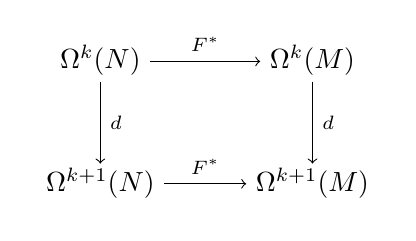
\begin{tikzpicture}
\matrix(m)[matrix of math nodes, row sep=3em, column sep=3em, text height=1.5ex, text depth=0.25ex]
{ \Omega^k(N)    &  \Omega^k(M)  \\
\Omega^{k+1}(N) &  \Omega^{k+1}(M)  \\};
\path[->,font=\scriptsize]
(m-1-1) edge node[auto]{$F^*$} (m-1-2)
edge node[auto]{$d$} (m-2-1)
(m-1-2) edge node[auto]{$d$} (m-2-2)
(m-2-1) edge node[auto]{$F^*$} (m-2-2);
%\path[right hook->](m-1-1) edge  node[auto]{$\,$} (m-2-1);
%\path[->,font=\scriptsize](m-1-2) edge  node[auto]{$p$} (m-2-2);
%edge node[auto]{$\gamma$} (m-2-2);
%\path[->,font=\scriptsize](m-1-2) edge  node[auto]{$p$} (m-2-2);
%\path[dashed,->,font=\scriptsize]
%(m-2-1) edge node[auto]{$G$} (m-1-2);
\end{tikzpicture}

So that 
\[
dF^* = F^* d
\]
%\end{proof}

 \hrulefill

define $\partial F(V) = F( \partial V)$ \\

generalized Stoke's thm.
\begin{equation}
        \int_{F(V)} d\beta^{p-1} = \int_{ \partial F(V)} \beta^{p-1} \quad \quad \quad (5.2)
\end{equation}

manifold needs only ``piecewise smooth'' boundaries.  



\subsection{ 5.2. Closed Forms and Exact Forms }

$\beta^p$ closed if $d\beta = 0$ \\ 
 $ \beta^p$ exact if $\beta^p = d\alpha^{p-1}$, some $\alpha^{p-1}$

\begin{theorem}[5.3] Let $M^n$ with 1st Betti number 0, $b_1 = 0$, i.e. $\forall \, $ closed oriented piecewise smooth curve $C$ is the boundary of some compact oriented ``surface''.  Then $\forall \, $ closed 1-form $\beta^1$ on $M^n$ is exact.
\end{theorem}

%\begin{proof}

\hrulefill \\


        Let $x,y \in M$, $y$ fixed.  \\
        oriented $C(y,x)$ starts at $y$, ends at $x$ 

define 
\[
f(x) \equiv \int_{C(y,x)} \beta^1
\]

If $\exists \, $ another $C^1(y,x)$, then $C- C'$ closed oriented curve.  

By given, $\exists \, $ oriented compact surface $F(V)$ s.t. $\partial F(V) = C$.  

\[
\int_C \beta - \int_{C'} \beta = \int_{C- C'} \beta = \oint_{ \partial F(V)} \beta = \int_{F(V)} d\beta = 0 
\]
$\int_C \beta = \int_{C'} \beta$.  $f$ independent of curve.  

Let $\mathbf{v}_x$ vector at $x$.  

Let vector field $\mathbf{v}$ coincide with $\mathbf{v}_x$ at $x$, defined in neighborhood of curve $C(y,x)$, $v=0$ at $y$.  

$\phi_t$ flow generated by $v$, $\phi_t C(y,x)$ curve joining $y$ to $\phi_i x$ 
\[
\begin{gathered}
        \left[ \frac{ d\phi_i x}{ dt} \right]_{t=0} = v_f \\ 
        df(v) = \frac{d}{dt} f\lbrace \phi_t x \rbrace_{t=0} = \left[ \frac{d}{dt} \int_{\phi_tC(y,x)} \beta \right]_{t=0} = \int_{ C(y,x) } \mathcal{L}_v \beta  = 
\end{gathered}
\]

\hrulefill

%\end{proof}

\subsection{ 5.3. Complex Analysis }




\subsubsection{5.5 Finding potentials}


\paragraph{5.5(1) Product of a closed and an exact form}\ \\
Let \ieq{\kappa} be a closed k-form and \ieq{\varepsilon} be an exact form with \ieq{\d\tilde\varepsilon=\varepsilon}. Then
\beq{
	\kappa\wedge\varepsilon
	&= \kappa\wedge\d\tilde\varepsilon
	 = (-1)^k(\d(\kappa\wedge\tilde\varepsilon)-\underbrace{\d\kappa}_{=0}\wedge\,\tilde\varepsilon)
	 = \d\left((-1)^k\kappa\wedge\tilde\varepsilon\right)
}


\section{6 Holonomic and Nonholonomic Constraints}

% 06Holonomic.tex

\subsection{6.1. The Robenius Integrability Condition}

Can one always find a surface orthogonal to a family of curves in $\mathbb{R}^3$?

\subsection{6.2. Integrability and Constraints}

\subsection{6.3. Heuristic Thermodynamics via Caratheodory}

Can one go adiabatically from some state to any nearby state?

\subsubsection{6.3a. Introduction}



\subsubsection{6.3b. The First Law of Thermodynamics}

Consider system of regions of fluids separated by ``diathermous'' membranes \\
\phantom{\quad \, } allow only passage of heat, not fluids \\

assume system connected \\
assume each state in thermal equilibrium

Let $p_i,v_i$ (uniform) pressure and volume of $i$th region \\
\phantom{\quad \, } at thermal equilibrium, ``equations of state'' $p_iv_i = n_iRT_i$ \\
\phantom{\quad \quad \, } $p_i v_i = n_iRT_i$ eliminate all but 1 pressure
\[
\Longrightarrow p_1, v_1,v_2, \dots v_n
\]
assume globally defined energy function $U$

path in $M^{n+1}$ represents sequence of states each in equilibrium, i.e. assume very slow changes in time, quasi-static irreversible processes, e.g. ``stirring'' \\
on $M$, $\text{dim}{M} = n+1$, assume $\exists \, $ work 1-form $W$, work done by system 
\[
W = p_i dv_i = p_i(U,v_1\dots v_n)dv_i \quad \quad \, i=1 \dots n 
\]
heat 1-form, heat added or removed from system, assume $Q \neq 0$
\[
Q = \sum_{i=0}^n Q_i(U,v_1 \dots v_n) dv_i \quad \, (v_0 = U)
\]

1st. law of thermodynamics 
\[
dU = Q-W
\]
energy conservation 

\subsubsection*{6.3c. Some Elementary Changes of State}

1. Heating at constant volume. 

\phantom{\quad \, } path $\gamma_I \in M$, $\text{dim}M = n+1$ s.t. $dv_1 = \dots = dv_n =0$.  $W=0$
\phantom{\quad \, } $dU = Q_0 dU$.  $\dot{\gamma}_I = c_0 \frac{\partial}{ \partial U}$

2. Quasi-static adiabatic process.  No heat exchanged,
\[
Q(\dot{\gamma}_{\text{II}}) = 0 \quad \, \text{ so } dU = -W
\]

3. Stirring at constant volume adiabatic, but not quasistatic  \\
\phantom{\quad \, } $Q,W$ makes no sense but \\
\phantom{\quad \, } work is being done by (or on) system, $U(y') - U(x)$, difference of internal energy \\
assume connected mechanical manifold $V$, $\text{dim}V =n$ \\
\phantom{assume } diff. $\pi:M \to V$ \\
\phantom{assume diff} $\pi$ onto \\
\phantom{assume diff} $\pi_*$ onto \\
\phantom{assume diff} $\pi$ submersion

By main thm. on submanifolds of Sec. 1.3d, \\
\phantom{\quad \, } if $v\in V$, then $\pi^{-1}(v)$ 1-dim. embedded submanifold of $M$ \\
\phantom{\quad \quad \, } assume $\forall \, \pi^{-1}(v)$ connected, we're assuming given any pair of states \\
\phantom{\quad \quad \quad \, } lying on $\pi^{-1}(v)$, 1 of them can be obtained by other by ``heating at constant volume''

assume $W$ on $M$ is $0$ when $\left. W \right|_{\pi^{-1}(v)} =0$ \\
on the other hand, $Q \neq 0$ on $\pi^{-1}(v)$; $dU = Q \neq 0$ (first law) \\
\phantom{\quad \, } $(U,v^1 \dots v^n)$ local coordinate system for $M$ ($U$ global coordinate)

\subsubsection{6.3d. The Second Law of Thermodynamics} 

cyclic process starts and ends at the same state

Kelvin 2nd. law of thermodynamics \\
\phantom{\quad \, } $\nexists $ quasistatic cyclic process can $Q$ converted entirely into $W$  \\

Caratheodory (1909) 2nd. law of thermodynamics \\
\phantom{\quad \, } $\forall \, $ neighborhood $N \ni $ state $x$, $\exists \, y$ not accessible from $x$ via quasistatic adiabatic paths, i.e. paths s.t. $Q=0$





\section*{II Geometry and Topology}

\section{$\mathbb R^3$ and Minkowski Space}
		
\subsection{7.1 Curvature and Special Relativity}

\subsubsection{7.1.a. Curvature of a Space Curve in $\mathbb{R}^3$}

$\mathbf{x} = \mathbf{x}(t)$ \, \quad $\left( \frac{ds}{dt} \right)^2 = v^2$ \, \quad $s(t) = \int_0^t \| \mathbf{x}(u) \| du$ \\
$\| \mathbf{v} \| = v$\[
\begin{aligned}
        & \dot{ \mathbf{x}} = \frac{d\mathbf{x}}{dt} = \mathbf{v} = \frac{d\mathbf{x}}{ds} \frac{ds}{dt} = \mathbf{T} v \\ 
        & \mathbf{a} = \ddot{x} = \mathbf{v} = \dot{v} \mathbf{T} + v\dot{\mathbf{T}} = \frac{d^2s}{dt^2} \mathbf{T} + v \frac{d\mathbf{T}}{ds} \frac{ds}{dt} = \dot{v} \mathbf{T} + v^2 \frac{d\mathbf{T}}{ds} \\ 
        & \mathbf{v} \times \mathbf{a} = v^3 \mathbf{T} \times \frac{d\mathbf{T}}{ds} = v^3 \kappa(s) \mathbf{T} \times \mathbf{n}
\end{aligned}
\]
so 
\[
\text{unit tangent vector } \mathbf{T} = \frac{d\mathbf{x}}{ds} = \dot{ \mathbf{x}} \left( \frac{dt}{ds} \right) = \frac{ \mathbf{v}}{v}
\]
Note that 
\[
\frac{d\mathbf{T}}{ds} \cdot \mathbf{T} = \frac{1}{2} \frac{d}{ds} \left( \mathbf{T} \cdot \mathbf{T} \right) = \frac{1}{2} \frac{d}{ds} (1) = 0 
\]

Now
\[
\frac{d\mathbf{T}}{ds} = \kappa(s) \mathbf{n}(s) \quad \quad \, (7.1)
\]
where $\mathbf{n}$ principal normal, $\kappa(s) \geq 0$ curvature of $C$.  
\[
\Longrightarrow \kappa = \frac{ \| \mathbf{v} \times \mathbf{a} }{v^3}
\]
\paragraph{7.1(1)}\ \\
\[
\begin{aligned}
        & x = \cos{\omega t} \\ 
        & y = \sin{\omega t} \\ 
        & z = kt 
\end{aligned} %\quad \quad \dot{x} = \left( \begin{matrix} - \omega s{\omega t}  \\ \omega c{\omega t} \\ k \end{matrix} \right) \quad \quad \mathbf{a} = \left( \begin{matrix} - \omega^2 c{\omega t} \\ - \omega^2 s{\omega t} \\ 0 \end{matrix} \right) \quad \, v = \sqrt{ \omega^2 + k^2} 
\]

\[
\mathbf{v} \times \mathbf{a} = \left| \begin{matrix} \mathbf{e}_x & \mathbf{e}_y & \mathbf{e}_z \\ -\omega s{\omega t} & \omega c{\omega t} & k \\ - \omega^2 c{\omega t} & - \omega^2 s{\omega t} & 0 \end{matrix} \right| = \left( \begin{matrix} k \omega^2 s{(\omega t)} \\ - k \omega^2 c{( \omega t)} \\ \omega^3 \end{matrix} \right)
\]
\[
\Longrightarrow \kappa = \frac{ \| \mathbf{v} \times \mathbf{a} \| }{v^3} = \frac{ \sqrt{ k^2 \omega^4 + \omega^6} }{ \sqrt{ ( \omega^2 + k^2)^3 } } = \frac{ \omega^2}{ \omega^2 + k^2 }
\]

\paragraph{7.1(2)}\ \\

Given $\mathbf{B} = \mathbf{T} \times \mathbf{n}$, 
\[
\frac{d\mathbf{B}}{ ds } = \frac{ d\mathbf{T} }{ds} \times \mathbf{n} + \mathbf{T} \times \frac{d\mathbf{n}}{ ds} = \mathbf{T} \times \frac{d\mathbf{n}}{ ds}
\]
so
\[
\mathbf{n} \times \frac{d\mathbf{B}}{ds} = \mathbf{n} \times (\mathbf{T} \times \frac{d\mathbf{n}}{ds} ) = \left( \mathbf{n} \times \frac{d\mathbf{n}}{ds} \right) \mathbf{T} - (\mathbf{n} \times \mathbf{T}) \frac{d\mathbf{n}}{ds} = 0 
\]
Indeed
\[
\begin{aligned}
        & \mathbf{T} \cdot \frac{d\mathbf{B}}{ds} = 0 \\ 
        & \mathbf{B} \cdot \frac{d \mathbf{B}}{ds} = \frac{d}{ds} ( \mathbf{B}\cdot \mathbf{B}) = \frac{d}{ds}(1)= 0 
\end{aligned}
\]

Then $\frac{d\mathbf{B}}{ds} \parallel \mathbf{n}$. \\

Define torsion $\frac{d\mathbf{B}}{ds} = \tau(s) \mathbf{n}$\\

Using $CAB-BAC$,
\[
\begin{gathered}
        \mathbf{n} \times \mathbf{B} = \mathbf{n} \times (\mathbf{T} \times \mathbf{n} ) = \mathbf{T} \\ 
        \mathbf{T} \times \mathbf{B} = \mathbf{T} \times (\mathbf{T} \times \mathbf{n} ) = (\mathbf{n} \cdot \mathbf{T} ) \mathbf{T} - ( \mathbf{T} \cdot \mathbf{T} ) \mathbf{n} = - \mathbf{n} \\
        \Longrightarrow \mathbf{n} = \mathbf{B} \times \mathbf{T}
\end{gathered}
\]

So
\[
\frac{ d \mathbf{n}}{ d s} = \frac{ d\mathbf{B}}{ds} \times \mathbf{T}  + \mathbf{B} \times \frac{ d\mathbf{T}}{ ds} = \tau \mathbf{n} \times \mathbf{T} + \mathbf{B} \times \kappa \mathbf{n} = \boxed{ - \tau \mathbf{B} + - \kappa \mathbf{T}  = \frac{ d \mathbf{n}}{ds} } 
\]


\subsubsection{7.2 Electromagnetism in Minkowski Space}

\paragraph{7.2(3)\quad Field strength 2-Form}\ \\
Notation: \ieq{\d x^0 = \d t}; \ieq{\d x^{ij\cdots} = \d x^i \wedge \d x^j \wedge \cdots}. The expansion for \ieq{*F} was taken from (14.20) combined with (3.41).
\beq{
	F \wedge F
		&= (E_i \d x^{i0} + B_{J=\{1,2,3\}} \d x^J) \wedge (E_k \d x^{k0} + B_{L=\{1,2,3\}} \d x^L) \\
		&= -E_iE_k \bcancel{\d x^{i0k0}} + B_JB_L \bcancel{\d x^{JL}} + E_iB_L \d x^{i0L} + B_JE_k \d x^{Jk0} \\
		&= -2 E_iB_J \d x^{0iJ} \\
		&= -2 (E_1B_{23}\d x^{0123} + E_2B_{13}\d x^{0213} + E_3B_{12}\d x^{0312}) \\
		&= -2 \underbrace{(E_1B_{23} + E_2B_{31} + E_3B_{12})}_{= \langle\vec E, \vec B\rangle}\underbrace{\d x^{0123}}_{= \vol^4} \\
		&= -2 \, \langle\vec E, \vec B\rangle \vol^4 \\
	F \wedge *F
		&= (E_i\d x^{i0}+B_{J=\{1,2,3\}}\d x^J) \wedge (-(\vec*B)_k\d x^{k0} + (\vec*E)_{L=\{1,2,3\}}\d x^L) \\
		&= - E_iB^{\vec*}_j \bcancel{\d x^{i0k0}} + B_JE^{\vec*}_L \bcancel{\d x^{JL}} + E_iE^{\vec*}_L\d x^{0iL} - B_JB^{\vec*}_k\d x^{0Jk} \\
		&= B^{\vec*}_kB_J \d x^{0kJ} - E_iE^{\vec*}_L \d x^{0iL} \\
		&= B^{\vec*}_kB_J \d x^{0kJ} - E_kE^{\vec*}_J \d x^{0kJ} \\
		&= (B^{\vec*}_kB_J - E_kE^{\vec*}_J) \d x^{0kJ} \\
			&\qquad\text{(permute k, J so their combination is in increasing order; } \\
			&\qquad\text{ permuting the double indices of B, E cancels out the minus)} \\
		&= (\|\vec B\|^2-\|\vec E\|^2) \vol^4
}


\section{The Geometry of Surfaces in $\mathbb{R}^3$}

\section{9 Covariant Differentiation and Curvature}
		\subsubsection{9.1 Covariant Differentiation}

\begin{definition}
affine connection or covariant differentiation is operator $\nabla (X,v) \mapsto \nabla_X v$ \quad \, $\begin{aligned} & \quad \\ 
       & \text{ vector $X$ at $p$ } \\ 
       & \text{ vector field $v$ at $p$ } \end{aligned}$

\begin{equation} 
\begin{gathered}
\nabla_X (av+ bw) = a\nabla_X v + b \nabla_X w \\ 
         \nabla_{ aX + bY} v = a\nabla_X v + b\nabla_Y v
\end{gathered} \quad \quad \quad (9.2)
\end{equation}

\[
\begin{gathered}
\nabla_X (fv) = X(f)v + f\nabla_X v  \quad \quad \, \text{(``Leibniz rule'')}
\end{gathered}
\]

demand if $X$ smooth, $\nabla_X v$ smooth vector field. 
\end{definition}

in our work up until now, we have always used local coordinates $x$ to yield a basis $\frac{ \partial}{ \partial x^i}$ for tangent vectors in a patch $U$.  

For many purposes, however, it is advantageous to use a more general basis.

frame of vector fields in $U$ - $n$ linearly independent smooth vector fields
\[
\mathbf{e} = (e_1 \dots e_n)
\]
coordinate frame = special case, $e_i = \frac{ \partial }{ \partial x^i}$ for some coordinate system $x$ in $U$

frame $\mathbf{e}$ usually not coordinate frame, since $[e_i, e_j]$ usually not 0 while $[\partial_i, \partial_j] =0$

\begin{theorem}[9.3] frame $\mathbf{e}$ is locally a coordinate frame iff
\[
[e_i , e_j] = 0 \quad \, \forall \, i,j
\]
\end{theorem}

% \begin{proof} (proof environment not defined)
Proof: 

We need only show that $[e_i, e_j]=0$ implies $\exists \, $ functions $(x^i)$ such taht 
\[
e_i = \frac{ \partial }{ \partial x^i }
\]

Let $\sigma$ be the dual form basis.  From (4.25)

\begin{equation}
d\sigma^i(e_j, e_k) = -\sigma^i([e_j, e_k]) \quad \quad \quad \, (9.4)        
\end{equation}




% \end{proof} (proof environment not defined)




Let $e = (e_1 \dots e_n)$ frame in $U$.  Then $X=e_j X^j$ 
\begin{equation}
\begin{aligned}
        \xrightarrow{ (9.2)} \nabla_X(e_k v^k) & = X(v^k) e_k + v^k \nabla_X e_k = X^j e_j v^k e_k + v^k X^j \nabla_{e_j} e_k = X^j e_j(v^k)e_k + X^j e_i \omega^i_{jk} v^k = \\ 
        & = X^j e_i \omega^i_{jk} v^k + X^j e_j(v^k)e_k 
\end{aligned} \quad \quad \quad (9.5)
\end{equation}

where $\omega^i_{jk}$ defined 

\begin{equation}
        \nabla_{e_j} e_k = e_i \omega^i_{jk} \quad \quad \quad (9.6)
\end{equation}

when $e_j = \partial_j$ coordinate frame, $\omega^i_{jk} = \Gamma^i_{jk}$

since $X(v^k) = dv^k(X)$

\[
\nabla_X v = e_i \lbrace dv^i(X) + X^j\omega^i_{jk} v^k \rbrace
\]

$\omega^i_{jk}$ coefficients of affine connection.  \\

using dual basis $\sigma$ of 1-forms,

\begin{equation}
        \nabla_X v = e_i \lbrace dv^i(X) + \omega^i_{jk} \sigma^j(X) v^k \rbrace = e_i \lbrace dv^i + \omega^i_{jk} \sigma^j v^k \rbrace(X) \quad \quad \quad (9.7)
\end{equation}

i.e.

\begin{equation}
\boxed{ \nabla_X v = dv(X) + \omega^i_{jk} + \omega^i_{jk} \sigma^j(X) v^ke_i }
\end{equation}


when frame $e$ is coordinate frame $e_i = \partial_i = \frac{ \partial }{ \partial x^i}$, \, $\sigma^i = dx^i$

\[
\nabla_X v = \partial_i \lbrace \frac{ \partial v^i}{ \partial x^j} + \omega^i_{jk} v^k \rbrace dx^j(X)
\]

i.e. 

\begin{equation}
        (\nabla_X v)^i = \left[ \frac{ \partial v^i}{ \partial x^j} + \omega^i_{jk} v^k \right] X^j \quad \quad \quad (9.8)
\end{equation}


since $\nabla_X v$ assumed to be vector, conclude

\begin{equation}
        \nabla_j v^i = \left. v^i \right|_j \equiv \frac{ \partial v^i}{ \partial x^j} + \omega^i_{jk} v^k \quad \quad \quad (9.9)
\end{equation}

form the components of a mixed tensor, covariant derivative of vector $v$.  




\subsubsection{9.3 Cartan's Exterior Covariant Differential}

\subsubsection{9.3c. Cartan's Structural Equations}


denote \\
row matrix  $ e \equiv (e_1 \dots e_n) $ \\
column $\sigma \equiv (\sigma^1 \dots \sigma^n )^T$ \\

$n \times n$ matrix of connection 1-forms $\omega = (\omega^i_{ \, \, j} )$ \\

column vector of torsion 2-forms $\tau = (\tau^1 \dots \tau^n)^T$


\subsubsection{9.3d. The Exterior Covariant Differential of a Vector-Valued Form}

$\alpha$ vector-valued $p$-form \\
locally,
$\alpha = e_i \otimes \alpha^i$, $\forall \, \alpha^i = a^i_{\, \, \underline{J}}(x) \sigma^J$ locally defined $p$-form \\

\textbf{exterior covariant differential}, vector-valued $(p+1)$ form $\nabla \alpha$ \\
\phantom{\quad } defined by Leibniz rule
\[
\nabla \alpha = \nabla (e_i \otimes \alpha^i) = (\nabla e_i) \otimes_{\wedge} \alpha^i + e_i \otimes d\alpha^i
\]
where
\[
(\nabla e_i)\otimes_{\wedge} \alpha^i = (e_k \otimes \omega^k_{\, \, i} ) \otimes_{\wedge} \alpha^i \equiv e_k \otimes (\omega^k_{\, \, i} \wedge \alpha^i)
\]

column of $p$ forms $\alpha = (\alpha^1 \dots \alpha^n)^T$

\begin{equation}
\nabla \alpha = e\otimes (d\alpha + \omega \wedge \alpha ) \quad \quad \quad \, (9.31)
\end{equation}


\paragraph{9.3(1) Basis expansion of the curvature form}
\beq{
	\tensor\theta{^i_j}
	&= \d\tensor\omega{^i_j} + \tensor\omega{^i_r}\wedge\tensor\omega{^r_j}
	 = \d\left(\tensor\omega{^i_{\ell j}}\d u^\ell\right) + \left(\tensor\omega{^i_{kr}}\d u^k\right)\wedge \left(\tensor\omega{^r_{\ell j}}\d u^\ell\right) \\
	&= \underbrace{\left(\partial_k\tensor\omega{^i_{\ell j}} + \tensor\omega{^i_{kr}}\tensor\omega{^r_{\ell j}}\right)}_{\identical\, \text{``}(_{k\ell})\text{''}} \underbrace{\d u^k\wedge\d u^\ell}_{\identical\, \d u^{k\ell}}
	 = \frac12 \left((_{k\ell})\d u^{k\ell} + (_{k\ell})\d u^{k\ell}\right) \\
	 	&\qquad\text{(In the second summand, commute the wedge product,} \\
	 	&\qquad\text{ afterwards rename }k\leftrightarrow \ell\text{)} \\
	 &= \frac12 \left((_{k\ell})\d u^{k\ell} - (_{\ell k})\d u^{k\ell}\right) \\
	 &= \frac12 \underbrace{\left(\partial_k\tensor\omega{^i_{\ell j}} - \partial_\ell\tensor\omega{^i_{kj}} + \tensor\omega{^i_{kr}}\tensor\omega{^r_{\ell j}} - \tensor\omega{^i_{\ell r}}\tensor\omega{^r_{kj}}\right)}_{=\tensor R{^i_{jk\ell}}} \d u^k\wedge\d u^\ell \\
	&= \frac12\tensor R{^i_{jk\ell}} \d u^k\wedge\d u^\ell
}



\paragraph{9.3(2) Covariant derivative of the identity form}
\beq{
	\vec\nabla\text{``}\d\vec r\text{''}
	&= \vec\nabla\left(\vec e_i \otimes \sigma^i\right)
	 = \vec e_i \otimes \underbrace{\left(\d\sigma^i + \tensor\omega{^i_j}\wedge\sigma^j\right)}_{=\tau^i}
	 = \vec e_i \otimes \tau^i
}
\emph{Remark:} The reason for calling \ieq{\vec e_i\otimes\sigma^i} the identity form is because
\beq{
	\vec e_i\otimes\sigma^i(\vec v)
	&= \vec e_i\otimes\sigma^i(v^j\vec e_j)
	 = \vec e_iv^j\underbrace{\sigma^i(\vec e_j)}_{=\delta^i_j}
	 = \vec e_iv^i
	 = \vec v
}











\subsubsection{9.4 Change of Basis and Gauge Transformations}




\paragraph{9.4(1) Transformation of the curvature form}\ \\
For readability, let \ieq{\bar P \equiv P^{-1}}.
\beq{
	   \theta'
	&= \d\omega' + \omega'\wedge\omega' \\
	&= \d(\bar P\omega P + \bar P\d P) \\
		&\qquad + (\bar P\omega P + \bar P\d P)\wedge(\bar P\omega P + \bar P\d P) \\
	&= \d(\bar P\omega P) + \d(\bar P\d P) \\
		&\qquad + \bar P\omega P\wedge\bar P\omega P + \bar P\omega P\wedge\bar P\d P + \bar P\d P\wedge\bar P\omega P + \bar P\d P\wedge\bar P\d P \\
	&= \d\bar P\wedge\omega P + \bar P\d\omega P - \bar P\omega\wedge\d P + \d\bar P\wedge\d P + \cancel{\bar P\d^2P} \\
		&\qquad + \bar P\omega P\wedge\bar P\omega P + \bar P\omega P\wedge\bar P\d P + \bar P\d P\wedge\bar P\omega P + \bar P\d P\wedge\bar P\d P \\
		&\qquad\text{(Use }0 = \d\unity = \d(\bar P P) = \d\bar P P + \bar P\d P \Leftrightarrow \d\bar P = -\bar P\d P\bar P \text{;} \\
		&\qquad\text{Also, the matrices ``commute'' with the wedge product, i.e. ``}A\wedge B=AB\wedge\text{'')} \\
	&= -\bar P\d P\wedge\bar P\omega P + \bar P\d\omega P - \bar P\omega\wedge\d P - \bar P\d P\wedge\bar P\d P \\
		&\qquad + \bar P\omega\wedge\omega P + \bar P\omega\wedge\d P + \bar P\d P\wedge\bar P\omega P + \bar P\d P\wedge\bar P\d P \\
	&= \bar P\d\omega P + \bar P\omega\wedge\omega P \\
	&= \bar P(\d\omega + \omega\wedge\omega) P \\
	&= \bar P\theta P
}

And this dear children is why indices should be left away. (Yes, it's the same exercise.)

\beq{
	   \theta'^i{}_j
	&= \d\omega'^i{}_j + \omega'^i{}_k\wedge\omega'^k{}_j \\
	&= \d(\bar P^i{}_l\omega^l{}_m P^m{}_j + \bar P^i{}_l\d P^l{}_j) \\
		&\qquad + (\bar P^i{}_l\omega^l{}_m P^m{}_k + \bar P^i{}_l\d P^l{}_k)\wedge(\bar P^k{}_n\omega^n{}_o P^o{}_j + \bar P^k{}_n\d P^n{}_j) \\
	&= \d(\bar P^i{}_l\omega^l{}_m P^m{}_j) + \d(\bar P^i{}_l\d P^l{}_j) \\
		&\qquad + \bar P^i{}_l\omega^l{}_m P^m{}_k\wedge\bar P^k{}_n\omega^n{}_o P^o{}_j + \bar P^i{}_l\omega^l{}_m P^m{}_k\wedge\bar P^k{}_n\d P^n{}_j \\
		&\qquad + \bar P^i{}_l\d P^l{}_k\wedge\bar P^k{}_n\omega^n{}_o P^o{}_j + \bar P^i{}_l\d P^l{}_k\wedge\bar P^k{}_n\d P^n{}_j \\
	&= \d\bar P^i{}_l\wedge\omega^l{}_m P^m{}_j + \bar P^i{}_l\d\omega^l{}_m P^m{}_j - \bar P^i{}_l\omega^l{}_m\wedge\d P^m{}_j + \d\bar P^i{}_l\wedge\d P^l{}_j + \cancel{\bar P^i{}_l\d^2P^l{}_j} \\
		&\qquad + \bar P^i{}_l\omega^l{}_m P^m{}_k\wedge\bar P^k{}_n\omega^n{}_o P^o{}_j + \bar P^i{}_l\omega^l{}_m P^m{}_k\wedge\bar P^k{}_n\d P^n{}_j \\
		&\qquad + \bar P^i{}_l\d P^l{}_k\wedge\bar P^k{}_n\omega^n{}_o P^o{}_j + \bar P^i{}_l\d P^l{}_k\wedge\bar P^k{}_n\d P^n{}_j \\
		&\qquad\text{(Use }0 = \d\delta^i{}_j = \d(\bar P^i{}_k P^k{}_j) = \d\bar P^i{}_k P^k{}_j + \bar P^i{}_k\d P^k{}_j \Leftrightarrow \d\bar P^i{}_j = -\bar P^i{}_k\d P^k{}_l\bar P^l{}_j \text{;} \\
		&\qquad\text{Also, the matrices ``commute'' with the wedge product, i.e. ``}A^i{}_k\wedge B^k{}_j=A^i{}_kB^k{}_j\wedge\text{'')} \\
	&= -\bar P^i{}_r\d P^r{}_s\wedge\bar P^s{}_l\omega^l{}_m P^m{}_j + \bar P^i{}_l\d\omega^l{}_m P^m{}_j - \bar P^i{}_l\omega^l{}_m\wedge\d P^m{}_j - \bar P^i{}_r\d P^r{}_s\wedge\bar P^s{}_l\d P^l{}_j \\
		&\qquad + \bar P^i{}_l\omega^l{}_m\wedge\omega^m{}_o P^o{}_j + \bar P^i{}_l\omega^l{}_m\wedge\d P^m{}_j \\
		&\qquad + \bar P^i{}_l\d P^l{}_m\wedge\bar P^m{}_n\omega^n{}_o P^o{}_j + \bar P^i{}_l\d P^l{}_k\wedge\bar P^k{}_n\d P^n{}_j \\
	&= \bar P^i{}_l\d\omega^l{}_m P^m{}_j + \bar P^i{}_l\omega^l{}_m\wedge\omega^m{}_n P^n{}_j \\
	&= \bar P^i{}_l(\d\omega^l{}_m + \omega^l{}_n\wedge\omega^n{}_m) P^m{}_j \\
	&= \bar P^i{}_l\theta^l{}_m P^m{}_j
}




\paragraph{9.4(2) Transformation of the curvature form}\ \\
The Transformation rule for basis vectors is
\beq{
	\vec e'=\vec eP \Leftrightarrow e'_i = e_j \tensor P{^j_i}
}
The transformation from cartesian to polar coordinates is given by
\beq{
	\matrixp{x\\y} &= \matrixp{x(r,\varphi)\\y(r,\varphi)} = \matrixp{r\cos\varphi\\r\sin\varphi} \\
	P &= \pdq{(x,y)}{(r,\varphi)} = \matrixp{\pdq xr & \pdq x\varphi \\ \pdq yr & \pdq y\varphi} = \matrixp{\cos\varphi & -r\sin\varphi \\ \sin\varphi & r\cos\varphi}
}
Using Mathematica to skip the annoying 2nd semester homework assignment parts of finding the inverse and calculating derivatives,
\beq{
	\d P &= \matrixp{-\sin\varphi\d\varphi & -\sin\varphi\d r-r\cos\varphi\d\varphi \\ \cos\varphi\d\varphi & \cos\varphi\d r-r\sin\varphi\d\varphi} \\
	P^{-1} &= \matrixp{\cos\varphi & \sin\varphi \\ -\frac1r\sin\varphi & \frac1r\cos\varphi}
}
Multiplying these two expressions yields, as desired,
\beq{
	\omega' = \cancel{P^{-1}\omega P} + P^{-1}\d P = \matrixp{0 & -r\d\varphi \\ \frac1r\d\varphi & \frac1r\d r}
}
Since \ieq{\theta=0}, \ieq{\theta'} vanishes as well. This is obvious from the transformation behavior of \ieq{\theta}; direct computation confirms this, as
\beq{
	   \theta'
	&= \d\omega'+\omega'\wedge\omega' \\
	&= \d\matrixp{0 & -r\d\varphi \\ \frac1r\d\varphi & \frac1r\d r} + \matrixp{0 & -r\d\varphi \\ \frac1r\d\varphi & \frac1r\d r}\wedge\matrixp{0 & -r\d\varphi \\ \frac1r\d\varphi & \frac1r\d r} \\
	&= \matrixp{\cancel{\d0} & \d(-r\d\varphi) \\ \d\left(\frac1r\d\varphi\right) & \cancel{\d\left(\frac1r\d r\right)}} + \matrixp{\cancel{0\wedge0} - \cancel{r\d\varphi\wedge\frac1r\d\varphi} & \cancel{0\wedge(-r\d\varphi)}-r\d\varphi\wedge\frac1r\d r \\ \cancel{\frac1r\d\varphi\wedge0} + \frac1r\d r\wedge\frac1r\d\varphi & \cancel{\frac1r\d\varphi\wedge(-r\d\varphi)} + \cancel{\frac1r\d r\wedge\frac1r\d r}} \\
	&= \matrixp{0 & -\d r\wedge\d\varphi \\ -\frac1{r^2}\d r\wedge\d\varphi & 0} + \matrixp{0 & \d r\wedge\d\varphi \\ \frac1{r^2}\d r\wedge\d\varphi & 0} \\
	&= \matrixp{0&0\\0&0}
}
This exercise made the advantage of the matrix notation clear: use the connection coefficients like normal matrices, only that you put a wedge in between their components' differential form ``factors''.



\subsubsection{}

\subsubsection{ Parallel Displacement and Curvature on a Surface}

When is parallel displacement independent of path?

We saw in Section 8.7 that parallel displacement of a vector between 2 pts. of a surface is path-dependent;  \\
This phenomenon is referred to as holonomy.

\begin{theorem}[9.61]
        Let $U\subset M^2$ compact in Riemannian surface with piecewise smooth boundary $\partial U$ \\
Assume $U$ covered by single orthonormal frame field $e$ (e.g. $U$ contained in coordinate patch) \\
Let unit vector $\mathbf{v}$ parallel translated around $\partial U$ \\
\quad $\mathbf{e}$ defined orientation.

Then angle $\Delta \alpha$ between $\mathbf{v}_0, \mathbf{v}_f$ is 
\[
\Delta \alpha = \iint K dS = \iint_U K \sigma^1 \wedge \sigma^2
\]
\end{theorem}

Proof. parametrize $\partial U$, let $T$ tangent, let $\alpha = \arccos{ \langle e_1, v \rangle }$ \\
Although $\alpha$ (like $\mathbf{v}$) is not single-valued on $\partial U$, $d\alpha = \left( \frac{ d\alpha}{ds} \right) ds$ well-defined.
\[
\Delta \alpha = \arccos{ \langle v_0, v_f \rangle } = \oint_{ \partial U} d\alpha
\]

For 
\[
\mathbf{v} = \mathbf{e}_1 \cos{\alpha} + \mathbf{e}_2 \sin{\alpha}
\]

then

\[
\begin{gathered}
        \nabla v = e(dv + \omega v) = e_1 (dv^1 + \omega_{12} v^2 ) + e_2 ( dv^2 + \omega_{21} v^1 ) = e_1 (-\sin{\alpha} d\alpha + \omega_{12} \sin{\alpha} ) + e_2 ( \cos{\alpha} d\alpha + \omega_{21} \cos{\alpha} ) = \\
        = (-e_1 \sin{\alpha} + e_2 \cos{\alpha} )( d\alpha - \omega_{12})
\end{gathered}
\]

To say that $v$ parallel displaced around $\partial U$ is to say \\
\quad $\nabla v(T) =0$, i.e. $d\alpha - \omega_{12} =0$ along $\partial U$  \quad (9.62)

\[
d \alpha(T) = \omega_{12}(T)
\]

Then 
\[
\begin{gathered}
        \Delta \alpha = \oint_{\partial U} d\alpha = \oint_{\partial U} \omega_{12} = \iint_U d\omega_{12} = \\
        = \iint_U \theta_{12} = \iint_U K \sigma^1 \wedge \sigma^2 
\end{gathered}
\]


\section{10 Geodesics}

\section{11 Relativity, Tensors, and Curvature}

\section{12 Curvature and Topology: Synge's Theorem}

\section{13 Betti Numbers and De Rham's Theorem}

\section{14 Harmonic Forms}

\section*{III Lie Groups, Bundles, and Chern Forms}


	\section{15. Lie groups}
		\subsection{15.1 Lie Groups, Invariant Vector Fields and Forms}

\subsubsection{15.1a Lie Groups}

Topological $GL(n,\mathbb{R})$ is an open subset of $\mathbb{R}^{n^2}$ and as such is a $n^2$-dim. manifold. \\
(cf. pp. 392) \\
\subsubsection*{Examples}
4. $G = Sl(n,\mathbb{R})$.  $Sl(n,\mathbb{R})$ subgroup of $Gl(n,\mathbb{R})$, $\text{det}{x} = 1$.  Prob. 1.1(3). Submanifold of $\text{dim}{Sl(n,\mathbb{R})} = n^2 - 1$ \\
5. $G = O(n)$, Sec. 1.1. Submanifold of $\text{dim}{\frac{n(n-1)}{2} }$.  \\
6. $G = U(n)$.  Sec. 1. submanifold of complex $n^2$ space or real $2n^2$ space.  \\
8. $G = T^n$ abelian group of diagonal matrices of form $z = \text{diag}{[e^{i\theta_1} \dots e^{i \theta_n}]}$ (15.2) \\
\phantom{8. } This group is topologically $S^1 \times \dots \times S^1$, $n$-torus.  Since circle connected, $T^n$ connected.  From this, $U(n)$ also connected!  

\subsubsection{15.1b. Invariant Vector Fields and Forms}

\subsection{15.2 One-parameter subgroups}





\paragraph{15.2(1) Generator of rotations}
\beq{
	   e^{\vartheta J}
	&= \sum_{k=0}^\inf \frac{\vartheta^kJ^k}{k!}
	 = \sum_{k=0}^\inf \frac{\vartheta^{2k}J^{2k}}{(2k)!} + \sum_{k=0}^\inf \frac{\vartheta^{2k+1}J^{2k+1}}{(2k+1)!}
	 = \sum_{k=0}^\inf \frac{\vartheta^{2k}(J^2)^k}{(2k)!} + \sum_{k=0}^\inf \frac{\vartheta^{2k+1}J(J^2)^k}{(2k+1)!} \\
	&= I\sum_{k=0}^\inf \frac{\vartheta^{2k}(-1)^k}{(2k)!} + J\sum_{k=0}^\inf \frac{\vartheta^{2k+1}(-1)^k}{(2k+1)!}
	 = I\cos\vartheta + J\sin\vartheta
}






\paragraph{15.2(2) Generator of A(1)}

\beq{
	X &= \matrixp{a&b\\0&0} \\
	X^2 &= \matrixp{a&b\\0&0}\matrixp{a&b\\0&0} = \matrixp{aa&ab\\0&0} = a\matrixp{a&b\\0&0} = aX \\
	\Rightarrow X^n &= \Cases{I & n=0\\a^{n-1}X & n>0}
}
\beq{
	\Rightarrow e^{tX}
	&= \sum_{k=0}^\inf \frac1{k!}t^kX^k
	 = I + \sum_{k=1}^\inf \frac1{k!}t^ka^{k-1}X
	 = I + \frac1aX\sum_{k=1}^\inf \frac1{k!}t^ka^k \\
	&= I + \frac1aX\left(\sum_{k=0}^\inf \frac1{k!}t^ka^k - \frac{t^0a^0}{0!}\right) 
	 = \matrixp{1&0\\0&1} + \matrixp{1&\frac ba\\0&0}e^{ta} - \matrixp{1&\frac ba\\0&0} \\
	&= \matrixp{e^{ta}&\frac bae^{ta}-\frac ba\\0&0}
}




\paragraph{15.3(1) Maurer-Cartan equations}

\beqN{
	   \d\sigma^U(\vec X_R,\vec X_S)
	&= \cancel{\vec X_R(\sigma^U(\vec X_S))} - \cancel{\vec X_S(\sigma^U(\vec X_R))} - \sigma^U([\vec X_R,\vec X_S]) \notag\\
	&= -\sigma^U(C^T_{RS}\vec X_T) = -C^U_{RS} \label{dsigma_maurer_cartan}
}
\beq{
	\Rightarrow \d\sigma^U = \frac12\d\sigma^U(\vec X_R,\vec X_S)\sigma^R\wedge\sigma^S \overset{(\ref{dsigma_maurer_cartan})}= -\frac12C^U_{RS}\sigma^R\wedge\sigma^S
}
\beq{
	\Rightarrow
	   0
	&= \d(\d\sigma^U)(\vec X_L,\vec X_M,\vec X_S) \\
	&\overset{\text{(4.27)}}= \vec X_L(\d\sigma^U(\vec X_M,\vec X_S)) - \vec X_M(\d\sigma^U(\vec X_L,\vec X_S)) + \vec X_S(\d\sigma^U(\vec X_L,\vec X_M)) \\
		&\qquad - \d\sigma^U([\vec X_L,\vec X_M],\vec X_S) + \d\sigma^U([\vec X_L,\vec X_S],\vec X_M) - \d\sigma^U([\vec X_M,\vec X_S],\vec X_L) \\
	&= \cancel{\vec X_L(-C^U_{MS})} - \cancel{\vec X_M(-C^U_{LS})} + \cancel{\vec X_S(-C^U_{LM})} \\
		&\qquad - \d\sigma^U(C^R_{LM}\vec X_R,\vec X_S) + \d\sigma^U(C^R_{LS}\vec X_R,\vec X_M) - \d\sigma^U(C^R_{MS}\vec X_R,\vec X_L) \\
	&= C^U_{RS}C^R_{LM} + C^U_{RM}C^R_{SL} + C^U_{RL}C^R_{MS}
}


\subsection{The Lie Algebra of a Lie Group}

\subsubsection{15.3a. The Lie Algebra}

\subsubsection{15.3b. The Exponential Map}

\begin{theorem}[15.27] map $\exp : g \to G$ sending $A \mapsto e^A$ diffeomorphism of some neighborhood of $0\in g$ onto neighborhood of $e \in G$.  
\end{theorem}

%\begin{proof}
Pf. \\
        vector $X \in g$ \\
        \[
\exp_*(X) = \left. \frac{d}{dt} (\exp{ tX}) \right|_{t=0} = \frac{d}{dt} \left. \left( 1 + tX + \frac{1}{2} t^2 X^2 + \dots \right) \right|_{t=0} = X
\]

$\exp{}_* : g \to g$ is the identity, $\exp{}$ local diffeomorphism by inverse function thm. (The Jacobian is nonsingular).   \\

If $G$ not a matrix group, \\
given $X$ at $e$, $e^{tX} = \exp{(tX)}$ curve through $e$ whose tangent vector at $t=0$ is vector $X$ (recall $e^{tX}$ is the integral curve through $e$ of left invariant vector field $X$).  \\
Thus $\exp_*{(X)} = X$
%\end{proof}

	\section{16. Vector Bundles in Geometry and Physics}
		\paragraph{16.3(1) Connection on a tensor product space}
\beq{
	   \vec\nabla_{\vec X}''\Lambda
	&= \vec\nabla_{\vec X}''(\vec e_a\otimes\vec e'_R\lambda^{aR})
	 = \vec\nabla_{\vec X}\vec e_a\otimes\vec e'_R\lambda^{aR} + \vec\nabla_{\vec X}(\vec e_a\otimes\vec e'_R\lambda^{aR}) \\
	&= \underbrace{X^i\vec e_b\omega^b_{ia}\otimes\vec e'_R\lambda^{aR}}_{b\leftrightarrow a} + \underbrace{\vec e_a\otimes\vec e_S'\omega^S_{iR}\lambda^{aR}X^i}_{S\leftrightarrow R} + \vec e_a\otimes\vec e_R'\underbrace{\d\lambda^{aR}X^i}_{=X^i\partial_i\lambda^{aR}} \\
	&= X^i\vec e_a\otimes\vec e_R'(\partial_i\lambda^{aR}+\omega^a_{ib}\lambda^{bR}+\omega^R_{iS}\lambda^{aS})
}


\section{17. Fiber Bundles, Gauss-Bonnet, and Topological Quantization  }
% 17fiberbundles.tex

\begin{quote}
  A vector bundle is a family of vector spaces parameterized by points in the base space. How do we parameterize a family of manifolds, say Lie groups?
\end{quote}

\section{ 17.1. Fiber Bundles and Principal Bundles }

\subsection{ 17.1a. Fiber Bundles }

\subsection{ 17.1b. Principal Bundles and Frame Bundles }

frame $\mathbf{e}$ at $p$ chosen

\begin{equation}
  f(p) = e_{\alpha}(p) g_{\alpha}(p) \quad \quad \quad \, (17.4)
\end{equation}

\begin{equation}
\begin{aligned}
  & \Phi_{\alpha} : U_{\alpha} \times G \to \pi^{-1}(U_{\alpha}) \\ 
  & \Phi_{\alpha}(p,g) = e_{\alpha}(p) g = (e_{\alpha})_i g^i_{ \, \, j } = f_j
\end{aligned}
\end{equation}

in an overlap, the same frame (17.4) will have another representation

\begin{equation}
  \mathbf{f}(p) = \mathbf{e}_{\beta}{(p)} g_{\beta}(p) \quad \quad \quad \, (17.5)
\end{equation}

\[
\begin{gathered}
  e_{\beta}(p) = e_{\alpha}(p) \tau_{\alpha \beta}(p) \\ 
  \tau_{\alpha \beta}(p) \equiv \tau_{\alpha \beta} \\ 
  g_{\alpha}(p) = \tau_{\alpha \beta}(p) g_{\beta}(p)
\end{gathered}
\]

diffeomorphism 
\[
\tau_{\alpha \beta}(p)  : G \to G
\]
left translation of $G$ by (transition) matrix $\tau_{\alpha \beta}(p)$



\subsection{ 17.1c. Action of the Structure Group on a Principal Bundle}

Let $\mathbf{f} = (\mathbf{f}_1 \dots \mathbf{f}_n)$ frame at $p$, $\mathbf{f} \in P$

\begin{theorem}[17.8]
  \[
(f \in P , g\in G) \to (fg) \in P 
\]
freely when $g\neq e$ and 
\[
\pi(fg) = \pi(f)
\]
i.e. preserves fibers
\end{theorem}

Proof:
  $\pi(\mathbf{f}) = p$ \\

$\Phi_{\alpha} : U_{\alpha} \times G \to \pi^{-1}(U_{\alpha})$ \quad \quad \, local trivialization \\
$\Phi_{\alpha}(p,g_{\alpha}) = \mathbf{f} \Longrightarrow \Phi_{\alpha}^{-1}(\mathbf{f}) = (p,g_{\alpha})$ 
\quad $\exists \, ! \, g_{\alpha}$ for $\mathbf{f}$

Let $g \in G$, 

right action of $g$ on $\pi^{-1}(U_{\alpha})$ is (locally action)

\[
\Phi_{\alpha}(p,g_{\alpha}g) = fg
\]

if $p \in U_{\alpha} \bigcap U_{\beta}$ 

\[
\begin{gathered}
  fg = \Phi_{\beta}(p,g_{\beta}g) = \Phi_{\beta}(p, \tau_{\beta \alpha}(p)g_{\alpha} g ) = \Phi_{\alpha}(p,g_{\alpha} g) 
\end{gathered}
\]
$\tau_{\beta \alpha} = \Phi_{\beta}^{-1} \Phi_{\alpha}$

\hrulefill

We see in this proof that the essential point is that \emph{left translations} in $G$ (say by $\tau_{\beta \alpha}$) \emph{ commute with right translations} (say by $g$).  



\subsection{ 17.2. }


\subsection{ 17.3. Chern's Proof of the Gauss-Bonnet-Poincar\'{e} Theorem }


\subsubsection{ 17.3a. A Connection in the Frame Bundle of a Surface }


\begin{equation}
  \omega \left( \frac{d\mathbf{x}}{dt} \right) \in \mathfrak{g} = \mathfrak{u}{ (1) } \quad \quad \quad \, (17.14)
\end{equation}










\section{18. Connections and Associated Bundles}

% 18ConnectionsandAssociatedBundles.tex

\subsection{ 18.1. Forms with Values in a Lie Algebra}

\begin{quote}
  What do we mean by $g^{-1} dg$?
\end{quote}

\subsubsection{ 18.1.a. The Maurer-Cartan Form }

If we think of $\omega$ as being a form that takes its values in the fixed vector space $\mathfrak{g}$, rather than as a matrix of 1-forms, we shall have an equivalent picture that is in many ways more closely related to the terminology used in physics.  

exterior form is differential form

\textbf{ Maurer-Cartan 1-form on $G$}

Let $\lbrace E_R \rbrace$ basis for $\mathfrak{g}$  \\
\phantom{Let} $\lbrace X_R \rbrace$ left invariant fields on $G$ obtained by left translating $E$'s  \\ 
\phantom{Let} $\lbrace \sigma^R \rbrace$ left invariant 1-forms on $G$ forming, $\forall \, g \in G$, basis dual to $\lbrace X_R \rbrace$  \\

$\sigma^R(X_S) = \delta^R_{ \, \, S}$

Then 
\begin{equation}
  \Omega \equiv E_R \otimes \sigma^R \quad \quad \quad \, (18.1)
\end{equation} 
\[
\Omega(Y_g) = E_R \sigma^R(Y_g) = E_R Y^R 
\]
$Y = X_R Y^R$ at $g\in G$, left translates back to 1

$\Omega : T_gG \to T_e G$

cf. Nakahara
\[
\Omega : Y \mapsto (L_{g^{-1}})_* Y = (L_g)^{-1}_* Y, \, Y \in T_g G
\]

Classically, Cartan wrote $\forall \, p \in M$, vector valued 1 form taking each $Y$ vector at $p$ into itself
\[
dp = \partial_i \otimes dx^i = \partial_i \otimes \delta^i_{ \, \, j }dx^j
\]
\begin{equation}
  \Omega = g^{-1} dg \quad \quad \quad \, (18.2)
\end{equation}

$dg$ takes $Y$ at $g$ into $Y$, $g^{-1}$ left transltates $Y$ back to $e$






\section{19. The Dirac Equation}

% 19TheDiracEquation.tex

\begin{quote}
Spin is what makes the world go 'round. -Theodore Frankel
\end{quote}

\subsection{19.1a. The Rotation Group $SO(3)$ of $\mathbb{R}^3$}

\[
\begin{aligned}
  & E_1 = \left[ \begin{matrix} & & \\ 
       & & -1 \\
      & 1 & \end{matrix} \right] \\
  & E_2 = \left[ \begin{matrix} & & 1 \\ 
       & &  \\
     -1  &  & \end{matrix} \right] \\
& E_3 = \left[ \begin{matrix} & -1 & \\ 
     1  & &  \\
      &  & \end{matrix} \right] 
\end{aligned}
\]
$(E_i)$'s are basis for $\mathfrak{so}(3)$

\[
[E_i,E_j] = \epsilon_{ijk}E_k
\]
$c_{ij}^k = \epsilon_{ijk}$

Consider 1-parameter group of rotations with angular velocity $\omega$, $\omega = \frac{d\theta}{dt}$

\[
\left. \frac{d \mathbf{r}}{dt} \right|_{t=0} = \omega \times \mathbf{r}(0)
\]

On the other hand, 1-parameter subgroup is of form $R(t) = e^{tS}$, $S$ skew-symmetric matrix
\[
\begin{gathered}
  r(t) = R(t)r(0) = e^{tS}r(0) \\ 
  \left. \frac{dr}{dt} \right|_{t=0} = Sr(0) \text{ so } S(r) = \omega \times r \\ 
 E_j(r) = e_j \times r
\end{gathered}
\]
\begin{equation}
R(t) = \exp{ (E_j \omega^jt)} \equiv \exp{ (E\cdot \omega t)} \quad \quad \quad \, (19.3) 
\end{equation}

\begin{equation}
R(\theta) = \exp{ (\theta E\cdot n ) } \quad \quad \quad \, (19.4)
\end{equation}



\subsection{19.1b. $SU(2)$: The Lie Algebra $\mathfrak{su}(2)$}

$\mathfrak{su}(2) = \mathfrak{g} = \lbrace X | X = - X^{\dag}; \text{tr}{(X)} = 0\rbrace$

$i\mathfrak{g} = \lbrace X | X = X^{\dag}; \text{tr}{(X)} = 0 \rbrace$, 

basis 
\[
\begin{aligned}
  & \sigma_1 = \left[ \begin{matrix} & 1 \\ 1 &   \end{matrix} \right] \\
  & \sigma_2 = \left[ \begin{matrix} & -i \\ i &   \end{matrix} \right] \\
  & \sigma_3 = \left[ \begin{matrix} 1 &  \\ & -1  \end{matrix} \right] \\
\end{aligned} \quad \quad \quad \, (19.5)
\]

\[
[ \sigma_j , \sigma_k ] = 2i \epsilon_{ijk} \sigma_i \quad \quad \quad \, (19.6)
\]

We shall see that $SU(2)$ simply connected.

Lie group theory states that $\exists \, $ homomorphism from $SU(2)$ onto $SO(3)$ \quad \, Pf. : Frobenius thm.

$\text{Ad}:SU(2) \to SO(3)$ \\
Claim: adjoint representation $\text{Ad}(g) = gYg^{-1}$ of $SU(2)$ on 3-dim. Lie algebra $\mathfrak{su}(2)$ yields (Thm. 19.2) standard representation of $SO(3)$ on $\mathbb{R}^3$

\[
\mathbf{x} = \mathbf{x} \cdot \mathbf{\sigma} = x^R \sigma_R = \left[ \begin{matrix} z & x - iy \\ x+ iy & - z \end{matrix} \right] = x_*
\]
inverse
\[
\begin{aligned}
  & x = \frac{1}{2} \text{tr}{ ( x_* \sigma_1 ) }  \\
  & y = \frac{1}{2} \text{tr}{ ( x_* \sigma_2 ) }  \\
  & z = \frac{1}{2} \text{tr}{ ( x_* \sigma_3 ) }  \\
\end{aligned} \quad \quad \quad \, (19.8)
\]

\[
\begin{aligned}
  & \mathbf{e}_1 = \left[ \begin{matrix} 1 \\ 0 \\ 0 \end{matrix} \right] \mapsto \sigma_1 \\ 
  & \mathbf{e}_2 = \left[ \begin{matrix} 0 \\ 1 \\ 0 \end{matrix} \right] \mapsto \sigma_2 \\ 
  & \mathbf{e}_3 = \left[ \begin{matrix} 0 \\ 0 \\ 1 \end{matrix} \right] \mapsto \sigma_3 
\end{aligned}
\]

$\mathbf{e}_i \cdot \sigma = \sigma_i$

real scalar product in $i\mathfrak{g}$ 
\[
\langle h, h' \rangle = \text{tr}(hh')
\]
as $\text{tr}{ (\sigma_j \sigma_k)} = 2\delta_{jk}$

Recall, $\forall \, $ Lie group $G$ acts on $\mathfrak{g}$ by adjoint action

\[
\begin{aligned}
  & \text{Ad}: G \to Gl(\mathfrak{g}) \\ 
  & \text{Ad}(g)(X) = gXg^{-1} \quad \quad \, \forall \, X \in \mathfrak{g}
\end{aligned}
\]

In this case, $SU(2) = \lbrace u | u^{\dag} u =1 \rbrace$, $\mathfrak{su}(2) = \lbrace X | X^{\dag} = -X, \text{tr}X \rbrace$, $\sigma_i$, $i=1,2,3$ basis for $\mathfrak{su}(2)$

\[
\begin{aligned}
  & \begin{aligned}
  & \text{Ad}: G \to Gl(\mathfrak{g}) \\ 
  & \text{Ad}(g)(X) = gXg^{-1} \quad \quad \, \forall \, X \in \mathfrak{g}
\end{aligned} \\
& \begin{aligned}
  & \text{Ad}: SU(2) \to \mathfrak{su}(2)  \\ 
  & \text{Ad}(u)(X) = uXu^{-1} \quad \quad \, \forall \, X \in \mathfrak{su}(2)
\end{aligned}
\end{aligned}
\]
Consider action of $SU(2)$ on $i\mathfrak{su}(2) = i\mathfrak{g}$ hermitian traceless matrices $X$. We'll still call this $\text{Ad}$

$\forall \, u \in SU(2)$ 
\[
\begin{aligned}
  & \text{Ad}(u) : i\mathfrak{g} \to i\mathfrak{g} \\ 
  & \text{Ad}(u) : i\mathfrak{su}(2) \to i\mathfrak{su}(2)
  & x_* \mapsto ux_*u^{-1} \quad \, \forall \, x_* \in i \mathfrak{su}(2)
\end{aligned}
\]

$\forall \, u \in SU(2)$, we're associated a $3\times 3$ matrix
\[
\text{Ad}(u) : \mathbb{R}^3 \to \mathbb{R}^3 \text{ using } (19.7) \begin{aligned}
  & \mathbb{R}^3 \to i\mathfrak{g} \\
  & x \mapsto x\cdot \sigma = x^R \sigma_R = x_* \end{aligned}
\]

Note $\text{Ad}$ is a representation of $SU(2)$ by $3\times 3$ matrices
\[
\text{Ad}(uu')(x_*) = uu'x_* (uu')^{-1} = \text{Ad}(u)\text{Ad}(u')x_*
\]
Note
\[
\langle \text{Ad}(u)x_* , \text{Ad}(u) x_* \rangle = \text{tr}(ux_*u^{-1}ux_*u^{-1}) \text{tr}(x_* x_*) = \langle x_* x_* \rangle
\]
so $\text{Ad}(u) \in O(3)$, $\text{Ad}$ representation of $SU(2)$ by orthogonal $3\times 3$ matrices.

\subsection{19.1c. $SU(2)$ is Topologically the 3-Sphere}

fundamental representation of $SU(2)$ by $2\times 2$ complex unitary matrices $uu^{\dag}=1$

$\left[ \begin{matrix} u_{11} & u_{12} \\ u_{21} & u_{22} \end{matrix} \right]$

Recall that the general form of $SU(2)$ matrices is the following: (cf. wikipedia)
\[
SU(2) = \lbrace \left( \begin{matrix} \alpha & - \overline{\beta} \\ \beta & \overline{\alpha} \end{matrix} \right) | \alpha , \beta \in \mathbb{C}, \, |\alpha|^2 + |\beta|^2 = 1 \rbrace
\]
$S^3 \subset \mathbb{C}^2 \approx \mathbb{R}^4$

\[
S^3 = \lbrace (z_1, z_2)^T | |z_1|^2 + |z_2|^2 = 1 \rbrace
\]
Note $SU(2) : S^3 \to S^3$ as $UU^{\dag}=1$ \quad \, $\forall \, U \in SU(2)$ i.e. (unitary) \\
Note $SU(2)$ acts transitively on $S^3$ \\


  Pf:
\[
\begin{gathered}
  (1,0)^T \in S^3 , \quad \quad \, u = \left[ \begin{matrix} z_1 & - \overline{z}_2 \\ z_2 & \overline{z}_1 \end{matrix} \right] \in SU(2) \\ 
 u\left( \begin{matrix} 1 \\ 0 \end{matrix} \right) = \left( \begin{matrix} z_1 \\ z_2 \end{matrix} \right) \quad \quad \, \forall \, \left( \begin{matrix} z_1 \\ z_2 \end{matrix} \right) \in S^3 \text{ i.e. (arbitrary) }
\end{gathered}
\]

So any $\left( \begin{matrix} z_1 \\ z_2 \end{matrix} \right) \in S^3$ can be ``reached'' from $\left( \begin{matrix} 1 \\ 0 \end{matrix} \right) \in S^3$ by some $u\in SU(2)$


From (17.10), topologically
\[
S^3 \approx \frac{SU(2)}{H}
\]
where $H$ is stability subgroup of pt. $\left( \begin{matrix} 1 \\ 0 \end{matrix} \right)$

But (19.11), $H = \lbrace 1 \rbrace$

\[
\Longrightarrow SU(2) \approx S^3
\]

In fact, 

\[
\begin{aligned}
  & SU(2) \to S^3 \\ 
  & u = \left( \begin{matrix} z_1 & - \overline{z}_2 \\ z_2 & \overline{z}_1 \end{matrix} \right) \mapsto \left( \begin{matrix} z_1 \\ z_2 \end{matrix} \right)
\end{aligned}
\]
In particular $SU(2) =S^3$ connected. \\
Since $\text{Ad}(u) \in O(3)$ orthogonal matrix, $\text{det}\text{Ad}(u) = \pm 1$ \\
since $u$ cont., and connected $S^3$, $\text{det}{ \text{Ad}(u)}= + 1$.  Thus $\text{Ad}{(u)} \in SO(3)$
\[
\text{Ad}:SU(2) \to SO(3)
\]

\subsection{$\text{Ad}:SU(2) \to SO(3)$ in More Detail}

\begin{theorem}[19.12]
representation $Ad:SU(2) \to SO(3)$ given in (19.10)
\begin{equation}
\begin{aligned}
  u \in SU(2) \\ 
  x_* \in i\mathfrak{su}(2) \\ 
  x_* \mapsto ux_* u^{-1} 
\end{aligned} \quad \quad \quad \, (19.10)
\end{equation}
is onto, i.e. $\forall \, $ rotation in $\mathbb{R}^3$, of form (19.10)


Furthermore, this representation is $2:1$, i.e. $\forall \, $ rotation $R$, $\exists \, $ exactly 2 $\pm u \in SU(2)$, s.t. $\text{Ad}(\pm u) = R$
\end{theorem}

EY : 20150217 What we have is this:

\[
\begin{aligned}
  \mathbb{R}^3 \overset{ \,_* }{=} \mathfrak{su}(2) \\ 
  (x,y,z) \overset{ \,_* }{ \mapsto } x^R \sigma_R
\end{aligned} \quad \quad \quad \, x_*^{-1}(X) = \frac{1}{2} ( \text{tr}(X\sigma_1 ), \text{tr}(X\sigma_2 ), \text{tr}(X\sigma_3 ) )^T
\]

\[
\begin{aligned}
  SU(2) \xrightarrow{ \text{Ad } } \text{Gl}(\mathfrak{su}(2)) \\ 
  u \mapsto \text{Ad}(u) \subset SO(3)
\end{aligned}
\]

\[
\begin{aligned}
  i\mathfrak{su}(2) \xrightarrow{ \text{Ad}(u) } i \mathfrak{su}(2) \\ 
  x_* \mapsto ux_* u^{-1}
\end{aligned}
\]


Pf: Let $u(t)$ 1-parameter subgroup of $SU(2)$ \\
\phantom{Pf: Let } $u(t) = \exp{ \left( \frac{t}{i} h \right)}$, $h$ $2\times 2$ hermitian matrix (i.e. $h=h^{\dag}$), $u(t) \in SU(2)$

$u(t) \to$ 1-parameter subgroup of $SO(3)$ under $ \begin{aligned}
  & \quad \\ 
  & i\mathfrak{su}(2) \to \mathbb{R^3} \\
  & x_* \overset{ \,_*^{-1}}{\mapsto} \mathbf{x} \end{aligned}$

\[
\text{Ad} u(t) \mathbf{x} \sim \text{Ad}u(t) x_* = e^{-ith} x_* e^{ith}
\]

\[
\begin{gathered}
  \left. \frac{d}{dt} \right|_0 \text{Ad}(u(t)) x_* = \left. \frac{d}{dt} \right|_0 e^{-ith} x_* e^{ith} = -i [h, x_* ] = -i [h^j \sigma_j, x^k\sigma_k] = -ih^jx^k[\sigma_j,\sigma_k] = -ih^jx^k \epsilon_{jki} \sigma^i(2i) =  \\
=  2\epsilon_{jki} h^jx^k\sigma^i   = 2(h\times x)^i\sigma_i
\end{gathered}
\]

EY : 20150217 Keep in mind 

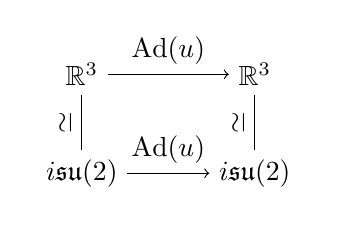
\begin{tikzpicture}
  \matrix (m) [matrix of math nodes, row sep=2em, column sep=3em, minimum width=1em]
  {
\mathbb{R}^3  & \mathbb{R}^3 \\
i\mathfrak{su}(2) & i \mathfrak{su}(2) \\ };
%  \path[-stealth]
  \path[->]
  (m-1-1) edge node [above] {$\text{Ad}(u)$} (m-1-2)
  (m-2-1) edge node [above] {$\text{Ad}{(u)}$} (m-2-2);
  \path[==]
  (m-1-1) edge node [above,rotate=90] {$\simeq$} (m-2-1)
  (m-1-2) edge node [above,rotate=90] {$\simeq$} (m-2-2);
\end{tikzpicture}

angular velocity vector of 1-parameter group $\text{Ad}u(t) x \in \mathbb{R}^3$ 
\[
\omega = 2h
\]

From (19.3)
\begin{equation}
  R(t) = \exp{ (E_j \omega^j t) } \equiv \exp{ (E\cdot \omega t) } \quad \quad \quad \, (19.3)
\end{equation}

\begin{equation}
\text{Ad}\exp{ \left( \frac{\sigma}{i} \cdot \mathbf{h}t \right)} x_* \sim R(t) \mathbf{x} = \exp{ (\mathbf{E} \cdot 2 \mathbf{h}t ) } \mathbf{x} \quad \quad \quad \, (19.13)
\end{equation}
or

\[
 i\mathfrak{su}(2) \xrightarrow{ \text{Ad}\exp{ \left( \frac{\sigma}{i} ht \right)} } i \mathfrak{su}(2)
\]

\[
\begin{gathered}
  i\mathfrak{su}(2) \to \mathbb{R}^3 \\ 
\boxed{   \text{Ad}\exp{\left( \frac{\sigma}{i} ht \right)}x_* \mapsto R(t) x = \exp{ (E\cdot 2ht) }x   }
% \frac{1}{2} ( \text{tr}{ (\text{Ad}\exp{\left( \frac{\sigma}{i} ht \right) } x_*\sigma_1 )} , \text{tr}{ (\text{Ad}\exp{\left( \frac{\sigma}{i} ht \right) } )} x_*\sigma_2 , \text{tr}{ (\text{Ad}\exp{\left( \frac{\sigma}{i} ht \right) } x_*\sigma_3  ) } )
\end{gathered}
\]

\begin{equation}
  \text{Ad}_*\left( \frac{\sigma_{\alpha} }{ 2i } \right)  = E_{\alpha} \quad \quad \quad \, (19.14)
\end{equation}

e.g. $h \in i\mathfrak{su}(2)$ \\
\phantom{e.g. } $h = \sigma_3$, $h = \left( \begin{matrix} 0 \\ 0 \\ 1 \end{matrix} \right)$

$t=\theta$

$u(t) \in SU(2)$
\[
u(t) = \exp{ \left( \frac{t}{i} h \right)} = \exp{ \left( \frac{t}{i} \sigma_3 \right)} = \left[ \begin{matrix} e^{-i\theta}  & \\ & e^{i\theta} \end{matrix} \right] = \exp{ \left( \frac{\theta}{i} \sigma_3 \right)}
\]
with $\sigma_3 = \left[ \begin{matrix} 1 & \\ & -1 \end{matrix} \right]$ \\

$\exp{ (E\cdot 2ht )} \in SO(3)$ 

\[
\overset{\text{Ad}_*\left( \frac{\sigma_{\alpha} }{2i} \right) }{ \mapsto } \exp{ (E\cdot 2h\theta)} = \exp{ (2\theta E_3)} = \exp{ \left[ \begin{matrix} & -2\theta & \\ 2\theta & & \\ & & \end{matrix} \right] } = \left[ \begin{matrix} \cos{2\theta} & -\sin{2\theta} & \\ \sin{2\theta} & \cos{2\theta} & \\ & & 1 \end{matrix} \right]
\]
with $\cdot h = E\cdot \sigma_3 = E_3 = \left[ \begin{matrix} & & -1 \\ & 1 & \\ & & \end{matrix} \right]$

For $SU(2)$, for $0\leq \theta 2\pi$, \\
$\exp{ \left( \frac{\theta \sigma_3}{i} \right) } $ is a simple closed curve, $\left[ \begin{matrix} e^{-i\theta} & \\ & e^{i \theta} \end{matrix} \right]$ \\

$\exp{ \left( 2\theta E_3 \right)}$ yields 2 full rotations \\

$\forall \, $ rotation of $\mathbb{R}^3$ is a rotation about some size, i.e. $R = \exp{ (E\cdot \omega \theta)} \in SO(3)$

By (19.13), 
\[
\text{Ad}\exp{ \left( \frac{\sigma}{i} \cdot h t \right) }x_* \mapsto R(t) x = \exp{ (E\cdot 2h t ) } = \exp{ ( E\cdot \omega \theta ) }
\]
So that 
\[
\text{Ad}\exp{ \left( \frac{\sigma}{2i} \cdot \omega \theta \right) } = R
\]
for 
\[
\begin{aligned}
  \omega = 2h \\ 
  E = \frac{\sigma}{2i}
\end{aligned}
\]
So \text{Ad} onto.  $\text{Ad}: SU(2) \to SO(3)$

If $\text{Ad}(u) = R$, $u=u(t) = \exp{ \left( \frac{t}{i} h \right)} \mapsto R = \exp{ (E\cdot \omega t)}$
\phantom{If }$\text{Ad}(u)x_* = ux_*u^{-1} \mapsto Rx$ \\ 
\phantom{If }$\text{Ad}(-u)x_* = u x_*u^{-1} \mapsto Rx$

So $\text{Ad}$ representation is at least $2:1$ i.e. not faithful \\

It's an elementary result of group theory that \\
\phantom{It's } if $\phi : G \to G'$ homomorphism of $G$ onto $G'$, then $G'$ isomorphic to coset $G/H$, where $H=\phi^{-1}(e')$ is kernel \\

(17.10) fundamental principle, $\forall \, G$ that acts on $G'$ by 
\[
(g,g') \mapsto \phi(g)g'
\]
and stability subgroup of $e'\in G'$ is kernel $H= \phi^{-1}(e')$ \quad \quad \, $\text{ker}{\phi} = H = \phi^{-1}(e')$ \\

$\text{Ad}:SU(2) \to SO(3)$ \quad \quad \, $\text{ker}{\text{Ad}} = \lbrace \pm 1 \rbrace$

(17.11) $\to SU(2)$ is fiber bundle over $SO(3)$; 
\[
\begin{aligned}
  & p^{-1} : SO(3) \to SU(2) \\ 
  & p^{-1}(R) \mapsto \lbrace \pm u \rbrace \text{ exactly 2 pts. }
\end{aligned}
\]

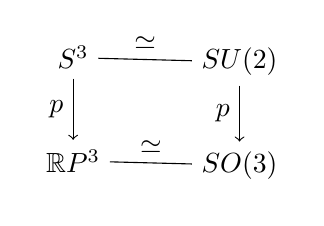
\begin{tikzpicture}
  \matrix (m) [matrix of math nodes, row sep=2em, column sep=3em, minimum width=1em]
  {
S^3  & SU(2) \\
\mathbb{R}P^3 & SO(3) \\ };
  \path[->]
  (m-1-1) edge node [left] {$p$} (m-2-1)
  (m-1-2) edge node [left] {$p$} (m-2-2);
  \path[==]
  (m-1-1) edge node [above,rotate=0] {$\simeq$} (m-1-2)
  (m-2-1) edge node [above,rotate=0] {$\simeq$} (m-2-2);
\end{tikzpicture}

$S^3/p = \mathbb{R}P^3$ \\
$\begin{aligned}
  & x\in S^3 \\
  & x\sim -x\end{aligned}$ \quad \, $[x] = \lbrace x,-x\rbrace$



\section{20. Yang-Mills Fields }

             % 20YangMillsFields.tex

\subsection{20.1. Noether's Theorem for Internal Symmetries }

\begin{quote}
\emph{How do symmetries yield conservation laws?}
\end{quote}

$\phi$ $N$-tuple $\phi^a(t,\mathbf{x}) = \phi^a(x)$, local representation of a section of some vector bundle $E$, 

\begin{tikzpicture}
  \matrix (m) [matrix of math nodes, row sep=2em, column sep=3em, minimum width=1em]
  {    
    E  &   \\     
    M &    \\ };
  \path[->]  (m-1-1) edge node [auto] {$\pi$} (m-2-1);
\end{tikzpicture}

%\begin{tikzpicture}
%  \matrix (m) [matrix of math nodes, row sep=2em, column sep=3em, minimum width=1em]
%  {
%    U_i \subset \mathbb{R}^{n+1} - 0 &  \\
%    V_i \subset \mathbb{R}P^n  & \mathbb{R}^n  \\ };
%  \path[-stealth]
%  (m-1-1) edge node [right] {$\varphi_i \pi$} (m-2-2)
%  edge node [left] { $\pi$} (m-2-1)
%  (m-2-1) edge node [below] {$\varphi$} (m-2-2);
%\end{tikzpicture}

In the case of a Dirac electorn, we have seen that $E$ is the bundle of complex 4-component Dirac spinors over a perhaps curved spacetime. If $E$ is not a trivial bundle (or if we insist on using curvilinear coordinates) we shall have to deal with the fact that $\partial_j \phi^a$ do not form a tensor.  

\subsubsection{ 20.1a. The Tensorial Nature of Lagrange's Equations }

Let $M^{n+1}$ (pseudo-) Riemannian manifold, let $E$ vector bundle over $M$; for definiteness, let fiber be $\mathbb{R}^N$. \\
section of this bundle over $U \subset M$ is described by $N$ real-valued functions $\lbrace \phi^a_U \rbrace$, \\
\quad where $\phi_V = c_{VU}\phi_U$ and \\
\quad \quad $c_{VU}(x)$ is $N\times N$ transition matrix function, $c^a_{VUb}$.   \\

notation $\begin{gathered} \quad \\
  \lbrace \Phi^a \rbrace \\ 
  \lbrace \Phi^a_{\alpha} \rbrace \\
\Phi^a_{\alpha} = \tau_{\alpha \beta} \Phi_{\beta} \end{gathered}$ \\

Lagrangian $L_0(x, \phi, \phi_x) \equiv L_0(x,\Phi, \partial_j \Phi^a)$



\subsection{20.2. Weyl's Gauge Invariance Revisited}

\subsubsection{ 20.2a. The Dirac Lagrangian }

\subsubsection{ 20.2b. Weyl's Gauge Invariance Revisited}

\subsubsection{ 20.2c. The Electromagnetic Lagrangian }

Instead of considering a change of (spacetime) coordinates $x$, we shall look at a change of the \emph{field} (fiber) coordinate $\psi$, i.e. \emph{a gauge transformation}.  

Since the phase of $\psi$ is not measurable, we \emph{should} be able to have invariance under a \emph{local} gauge transformation, where $\alpha = \alpha(x)$ varies with the spacetime point $x$!  \\
\quad Clearly the Dirac equation and Lagrangian are \emph{not} invariant under such a substitution because of the appearance of terms involving $d\alpha$.  \\
\quad It must be that \emph{there is some background field that is interacting with the electron}.  This background field will manifest itself through the appearance of the connection.  






\subsection{ The Yang-Mills Nucleon }

\begin{quote}
  How did the groups $SU(2)$ and $SU(3)$ appear in particle physics?
\end{quote}



\subsubsection{ 20.3a. The Heisenberg Nucleon }

\subsubsection{ 20.3b. The Yang-Mills Nucleon }

\subsubsection{ 20.3c. A Remark on Terminology }

We have related the connection matrices $\omega$ to the gauge potentials $A$ by 
\[
\omega = -i q A
\]
$q$ is called a generalized \textbf{charge}.  






\section{21.}









\begin{appendix}

\section{A. Elasticity}


\subsection{A.a. The Classical Cauchy Stress Tensor and Equations of Motion}

$B(t)$ compact body, might be portion of larger body in motion

mass 3 form 
\[
m^3 \equiv \rho \text{ vol }
\]

mass conservation
\[
\frac{d}{dt} \int_{B(t)} m^3 = \int_{B(t)} \mathcal{L}_{\textbf{v} + \frac{ \partial }{ \partial t}} m^3 = 0 
\]
$\mathbf{b}$ external force density (per unit mass)
\[
\frac{d}{dt} \int_{B(t)} v^i m^3 = \int_{B(t)} b^i m^3 + \int_{ \partial B(t)} t^{ij}n_j da
\]

\subsection{A.b. Stresses in Terms of Exterior Forms}

$t$ pseudo $(n-1)$ form on $M^n$ with values in tangent bundle $TM$ (vector bundle language)

\begin{equation}
        \mathbf{t} = \mathbf{e}_r \otimes \mathfrak{t}^r \equiv \mathbf{e}_r \otimes \mathfrak{t}^r_{ \, \, \underline{J}} \sigma^J 
\end{equation}

\[
\int_{ \partial B} \mathbf{t} = \int_{\partial B} \mathbf{e}_r \otimes \mathfrak{t}^r = \mathbf{e}_r \int_{\partial B} \mathfrak{t}^r = \mathbf{e}_r \int_{ \partial B} \mathfrak{t}^r_{ \underline{J}} dx^J
\]
as total traction that part of body outside $\partial B$ exerts on $B$

(2.73) $\forall \, $  Riemannian $M$, write $(n-1)$ form $\mathfrak{t}^r$ in terms of vector $t^{(r)}$

\[
\mathfrak{t}^r = i(\mathbf{t}^r) \text{vol} = i (\mathbf{t}^{(r)} ) \sqrt{g} \epsilon_{\underline{I}} dx^I = \sqrt{g} \mathbf{t}^{(r)i} \epsilon_{i \underline{J}} dx^J
\]

\begin{equation}
t^r_{ \, \underline{J}}  = \sqrt{g} t^{(r)i} \epsilon_{i \underline{J}} \quad \quad \, (A.6)
\end{equation}
\[
t^{ri} \equiv t^{(r)i} = \frac{1}{\sqrt{g}} t^r_{ \, \, \underline{J}} \epsilon^{i J }
\]
relation between stress form $t^r$ and Cauchy's stress tensor $t^{ri}$

assuming $\mathbf{t} = \mathbf{e}_r \otimes \mathfrak{t}^r$ is $(n-1)$ form section of the tangent bundle, thus from (9.31), we have

20141102 EY recall 
\[
\nabla \alpha = e \otimes (d\alpha + \omega \wedge \alpha) \quad \quad \quad \, (9.31)
\]
and 
\[
\begin{gathered}
        \nabla \alpha = \nabla( e_i \otimes \alpha^i) = (\nabla e_i) \otimes_{\wedge} \alpha^i + e_i \otimes d\alpha^i \\ 
 \text{ where }  \\
(\nabla e_i) \otimes_{\wedge} \alpha^i = (e_k \otimes \omega^k_{\, \, i}\otimes_{\wedge} \alpha^i \equiv e_k \otimes ( \omega^k_{\, \, i} \wedge \alpha^i)
\end{gathered}
\]

\begin{equation}
        \nabla t = \nabla (\mathbf{e}_r \otimes \mathfrak{t}^r) = \nabla \mathbf{e}_r \otimes_{\wedge} \mathfrak{t}^r + \mathbf{e}_r \otimes d\mathfrak{t}^r = \mathbf{e}_r \otimes (d\mathfrak{t}^r + \omega^r_{ \, \, s} \wedge \mathfrak{t}^s) = \mathbf{e}_r \otimes \nabla \mathfrak{t}^r \quad \quad \quad \, (A.7)
\end{equation}


\subsection{A.f. Hamilton's Principle in Elasticity}


\begin{equation}
        \delta U = \int_B \delta E_{RC} dX^R \wedge S^C \quad \quad \quad \, (A.24) 
\end{equation}

\begin{equation}
        \delta U = \int_B S^{CR} \delta E_{RC} \text{VOL}^n \quad \quad \quad \, (A.25)
\end{equation}

Hamilton's principle
\begin{equation}
\delta \int T dt - \int \delta U dt + \int \delta W dt = 0 \quad \quad \quad \, (A.26)
\end{equation}

We don't write $\delta \int U dt $ because we don't assume \\

We don't assume that $\exists \, $ stored energy function $U$ so we don't write $\delta \int U dt$, $\exists \, $ only differential $\delta U$

\end{appendix}
\end{document}
